\rhead[\thepage]{\scriptsize{CAPÍTULO \thechapter}. \rightmark}
\lhead[CAPÍTULO \thechapter. \leftmark]{}
%======================================================================
\chapter{Funciones matemáticas}
\label{FM}
\markboth{Funciones matemáticas}{Funciones matemáticas}
%======================================================================
Usualmente, se necesita agrupar elementos bajo ciertas condiciones como lo vimos en la sección (\ref{TC}). Ahora, hay ciertos grupos que tienen una correspondencia que asocia estos conjuntos, entonces se genera una dependencia del valor de un conjunto con respecto a otro, a esto se le llama \textit{función matemática}. 
\begin{mydef}
\textbf{Función matemática. }Una función de un conjunto $X$ a un conjunto $Y$ es una regla de correspondencia que asigna a cada elemento $x$ de $X$ exactamente un elemento $y$ de $Y$.
\end{mydef}

A las funciones se le acostumbra asignar letras como $f$, $g$ o $h$, pero puede ser cualquier letra o símbolo. La primera notación que usualmente se utiliza es $f:X\longrightarrow Y$ que nos dice desde donde y hasta donde va la función. En este caso va desde el conjunto $X$ que se llama \textit{dominio} hasta el conjunto $Y$ que se llama \textit{imagen} o \textit{recorrido}. La segunda forma de representar la función es $y=f(x)$, donde $y$ es un elemento de la imagen y $x$ es una elemento del dominio que se le aplicó la función $f()$.\\
La aplicación de una función se puede asemejar a un proceso que tiene entradas (los elementos $x$ del conjunto $X$), una función y salidas (los elementos $y$ del conjunto $Y$) con la función aplicada. Las entradas $x$ no dependen de nada previo, por lo que se les llama variables independientes y como las salidas $y$ dependen de las entradas se les llama variables dependientes.\\

La variable que aparece dentro del paréntesis en $f()$ es la que se reemplaza cada vez que aparezca la variable, es decir, si la función es $f()=()+3$ y uno desea saber la expresión de $f(j^{3})=j^{3}+3$.\\
\begin{myexample}
Evaluar una función con un elemento del dominio.
\begin{eqnarray*}
f(x)&=&x^{4}+3x^{2}+x+56\\
f(7)&=& (7)^{4}+3\cdot (7)^{2}+(7)+56=2611
\end{eqnarray*}
\end{myexample}

\begin{center}
\begin{figure}[h!]
\centering
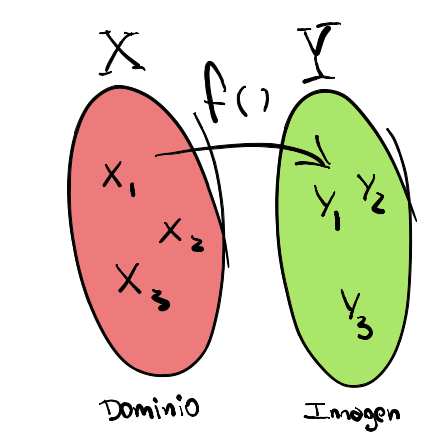
\includegraphics[scale=0.45]{function.png}
\caption[Esquema de una función matemática.]{Esquema de una función matemática. El óvalo rojo representa el dominio de la función que es un conjunto $X$ con los elementos $x_{1}$, $x_{2}$ y $x_{3}$. La flecha muestra la dirección de la función y la operación que se aplicará. El óvalo verde representa la imagen de la función de un conjunto $Y$ con elementos $y_{1}$, $y_{2}$ y $y_{3}$.}
\label{fn00}
\end{figure}
\end{center}

\begin{center}
\begin{figure}[h!]
\centering
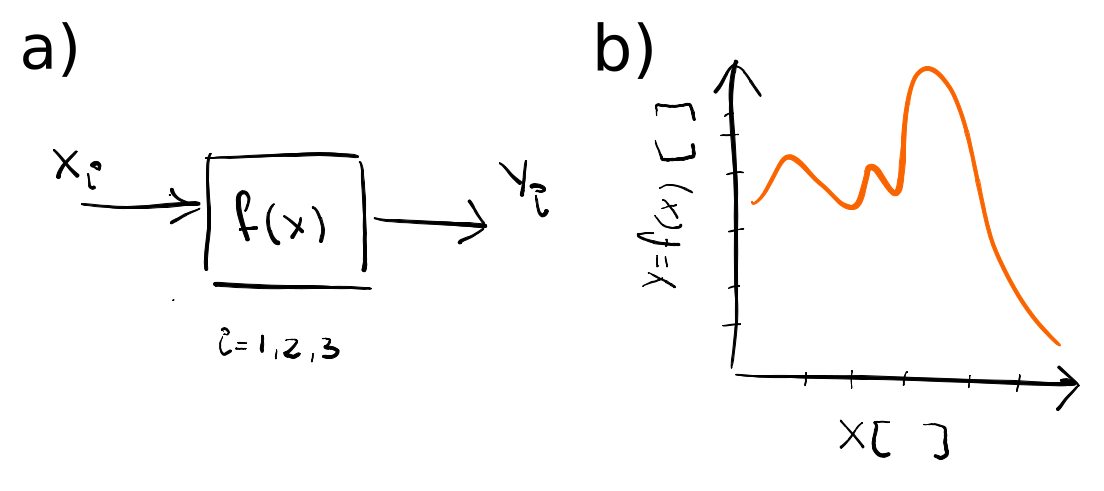
\includegraphics[scale=0.45]{function0.png}
\caption[Esquema de una función y gráfico de una variable dependiente e independiente.]{Esquema de una función y gráfico de una variable dependiente e independiente. a) Las variables $x_{i}$ representan las entradas de la función. Luego, la caja es donde se aplica la función $f(x)$ y finalmente se tiene una salida que son las variables $y_{i}$. b) Gráfica de una variable independiente, $x$, y una variable dependiente, $y$, que va cambiando su valor cuando se evalúa cada elemento del dominio (los $x_{i}$).}
\label{imagfx}
\end{figure}
\end{center}

%----------------------------------------------------------------------
\section{Dominio e imagen de una función}
\label{domim}
%----------------------------------------------------------------------
\begin{mydef}
\textbf{Dominio de una función.} El dominio de una función $f$ es el mayor subconjunto de números reales para los que $f(x)$ es un número real. Se denota $Dom(f(x))$.
\begin{eqnarray}
Dom(f(x))=\{x\in X|\exists y \in Y,f(x)=y\}
\end{eqnarray}
\label{domfx}
\end{mydef}
Entonces, el dominio de una función es el conjunto más grande donde está definida, por ejemplo $1/x$ está definido en para cualquier número real menos para el cero, por lo que el dominio de la función son todos los números reales menos el cero ($\mathbb{R}-\{0\}$). La imagen de la función son todos los valores que puede tomar $f(x)$.

\begin{mydef}
\textbf{Imagen de una función.} Es el conjunto $Y$ que tiene como elementos todos los posibles valores que puede tomar la función. Se denota como $Im(f(x))$.
\begin{eqnarray}
Im(f(x))=\{y\in Y|\exists x\in X,f(x)=y \}
\end{eqnarray}
\label{imfx}
\end{mydef}

\begin{myexample} Encontrar el dominio de las siguientes funciones:\\

\noindent\textit{i)}
\begin{eqnarray*}
f(x)&=&\sqrt{x+7}\\
Dom(f(x))&=& x+7\geq 0\\
Dom(f(x))&=& x\geq -7\\
Dom(f(x))&=& [-7,+\infty [
\end{eqnarray*}

\noindent\textit{ii)}
\begin{eqnarray*}
f(x)&=&\dfrac{1}{x^{2}-4}\\
Dom(f(x))&=& x^{2}-4\neq 0 \\
Dom(f(x))&=& x^{2}\neq 4 \\
Dom(f(x))&=& \sqrt{x^{2}}\neq \sqrt{4} \\
Dom(f(x))&=& |x|\neq 2 \\
Dom(f(x))&=& x\neq \pm 2 \\
Dom(f(x))&=& \mathbb{R}-\{-2,+2\}
\end{eqnarray*}
\end{myexample}

Para calcular el dominio de una función no hay un procedimiento único, por lo que se debe analizar el tipo de función que tenemos y que no se anule para que tome siempre valores reales. Por ejemplo, en el caso de las raíces cuadradas se debe cumplir que el radicando debe ser mayor que cero o para el caso de las expresiones fraccionales, el denominador debe ser distinto de cero. A continuación cual es el dominio de cierto tipo de funciones.

\begin{itemize}
	\item Funciones polinomiales: El dominio son todos los números reales.
	\begin{eqnarray*}
	f(x)&=&4x^{7}+50x^{25}+2\\
	Dom(f(x))&:& \mathbb{R}
	\end{eqnarray*}
	\item Función racional (fracciones): Son todos los números reales, menos los valores que hace cero al denominador.
	\begin{eqnarray*}
	f(x)&=&\dfrac{1}{x+2}\\
	Dom(f(x))&:&\mathbb{R}-\{-2\}
	\end{eqnarray*}
	\item Funciones radicales con índice par: El dominio son todos los valores que hacen que el radicando sea mayor que cero.
	\begin{eqnarray*}
	f(x)&=&\sqrt{3x+7}\\
	Dom(f(x))&:& \left[\dfrac{-7}{3},+\infty \right[
	\end{eqnarray*}
	\item Funciones radicales con índice impar: Es el dominio del radicando, no está sujeta a una desigualdad.
	\begin{eqnarray*}
	f(x)&=&\sqrt[3]{7x+3}\\
	Dom(f(x))&:& \mathbb{R}
	\end{eqnarray*}
	\item Función logarítmica: El dominio está formado por todos los valores que hacen que el argumento del logaritmo sea mayor que cero.
	\begin{eqnarray*}
	f(x)&=&log\left(2x^{2}+3x+1\right)\\
	Dom(f(x))&:& \left]-\infty ,-1\right[ \cup \left]-\dfrac{1}{2},\infty \right[
	\end{eqnarray*}
	\item Función exponencial: El dominio son todos los reales, excepto los valores que anulan a la función que está en el exponente.
	\begin{eqnarray*}
	f(x)&=&e^{x}\\
	Dom(f(x))&:&\mathbb{R}
	\end{eqnarray*}
	\begin{eqnarray*}
	f(x)&=&e^{1/x}\\
	Dom(f(x))&:&\mathbb{R}-\{0\}
	\end{eqnarray*}
\end{itemize}

\section{Gráficas de una función}
Al momento de plasmar una función cualquiera debemos juntar las definiciones de dominio (\ref{domfx}), imagen (\ref{imfx}) y la figura (\ref{imagfx}), con estos tres elementos podemos graficar una función. Cada punto de la gráfica tiene la forma $(x_{i},y_{i})$ o $(x_{i},f(x_{i}))$, por lo que el eje $x$ representa el dominio de la función y el eje $y$ la imagen. \\
La función para un valor $y$ puede tener más de un valor en $x$, por ejemplo en $x^{2}$. No se puede dar el caso inverso, es decir, que por un valor de $x$ la función tenga dos o más valores en el $y$, es por ello que si uno traza una línea vertical en las gráficas, esta línea debe tocar solo un punto del gráfico, si no, no es una función.\\

\begin{center}
\begin{figure}[h!]
\centering
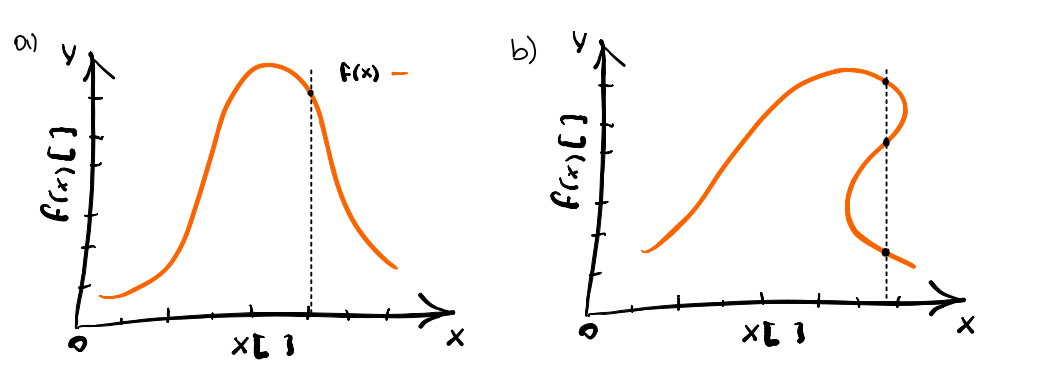
\includegraphics[scale=0.5]{lineafn.png}
\caption[Gráfica para diferenciar una función.]{Gráfica para diferenciar una función. a) Es una gráfica que muestra una línea vertical que toca en un solo punto a la gráfica, por lo tanto, es una función. b) La gráfica no es una función, ya que la línea toca a la función en tres puntos.}
\label{difx}
\end{figure}
\end{center}
Si la línea solo debe tocar en un punto, entonces ¿Qué ocurre cuando se grafica un círculo? En casos de círculos o elipses son dos funciones que al momento de graficarlas al mismo tiempo forman la figura. Por ejemplo, las gráficas que forman un círculo de radio 3 son $y=\pm\sqrt{9-x^{2}}$. 

\subsection{Intersecciones con los ejes}
Una de las formas más rápidas de obtener información de la gráfica de la función es ver en que puntos pasa por los ejes, se debe ver que para las intersecciones en el eje $y$ son de la forma ($0,f(0)$) mientras que para los del eje $x$ son ($x,0$). De esto se desprende que hay ciertos valores de $x$ que hacen que $y=0$, entonces el objetivo es encontrar esos $x$ que hace que $f(x)=0$. \\
Cuando se encuentran esos números se le llaman \textit{raíces} o \textit{soluciones} de la función que satisfacen la ecuación $f(c)=0$, siendo $c$ los números reales que son solución de la función.\\

Como se puede notar no siempre las funciones pasan por los ejes, hay casos en que la función toca en un solo punto, pero no cruza, a esto se llama una gráfica \textit{tangente} al eje. La función solo puede pasar o tocar al eje $y$ en un solo punto, siempre y cuando el $0$ esté en el dominio de la función.\\ 

\begin{center}
\begin{figure}[h!]
\centering
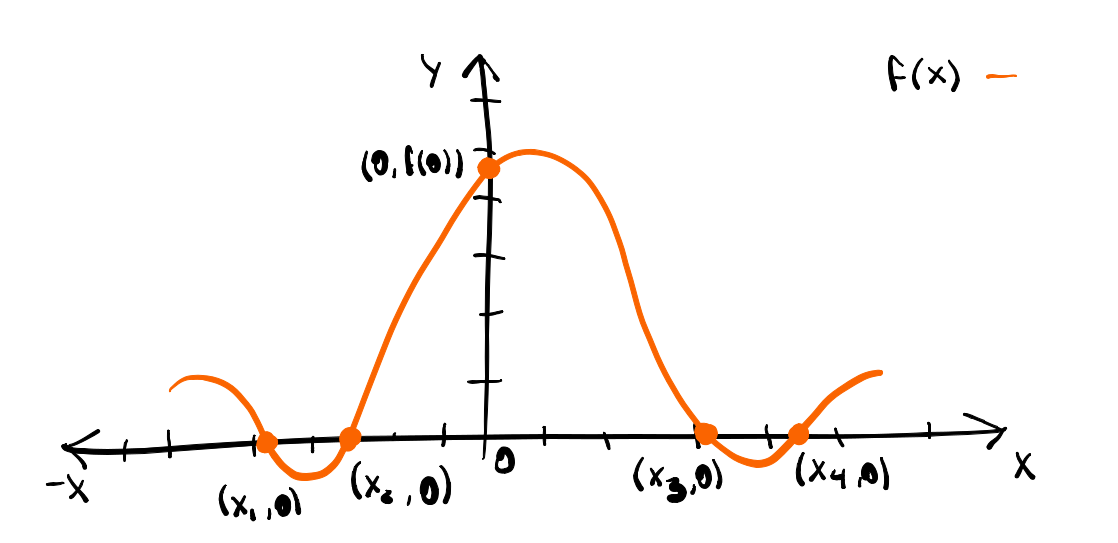
\includegraphics[scale=0.35]{interfn.png}
\caption[Función que intersecta los ejes.]{Función que intersecta los ejes. La función intersecta en 5 puntos y a los que pasan por el eje $x$ se les denomina ceros de la función. }
\label{interfx}
\end{figure}
\end{center}

\subsection{Simetrías y transformaciones }
El primer paso fue encontrar los puntos de intersección con los ejes, lo siguiente es identificar ciertos tipos de funciones para ver de forma rápida su gráfica en el plano. Hay ciertas funciones que tienen una invarianza\footnote{Es algo que no cambia al aplicarle una transformación.} que la llamaremos \textit{simetrías}. Todo esto al momento de ver la gráfica se ve que la función tiene un eje de simetría con respecto a un eje o recta.\\
Por la figura (\ref{imagfx}) se ve que la función solo puede tener simetría con respecto al eje $y$ (o una traslación del mismo), porque en caso contrario no sería una función. Esta simetría se puede clasificar en dos tipos, funciones \textit{pares} e \textit{impares}.
\begin{mydef}
\textbf{Funciones pares e impares.} Sea $x$ y $-x$ elementos perteneciente al dominio de la función $f(x)$. Se dice que:\\
\noindent i) Una función $f$ es par si $f(-x)=f(x)$.\\
\noindent ii) Una función $f$ es impar si $f(-x)=-f(x)$.\\
\end{mydef}


\begin{myexample}
Funciones pares e impares:\\

\noindent i) Función par:\\
\begin{eqnarray*}
f(x)&=&x^{2}\\
f(-2)&=&(-2)^{2}=4\\
f(2)&=&(2)^{2}=4\\
f(x)&=&f(-x)\\
\end{eqnarray*}
\noindent ii) Función impar:\\
\begin{eqnarray*}
f(x)&=&x^{3}\\
f(-2)&=&(-2)^{3}=-8\\
f(2)&=&(2)^{3}=8\\
f(x)&=&-f(x)
\end{eqnarray*}
\end{myexample}

\begin{center}
\begin{figure}[h!]
\centering
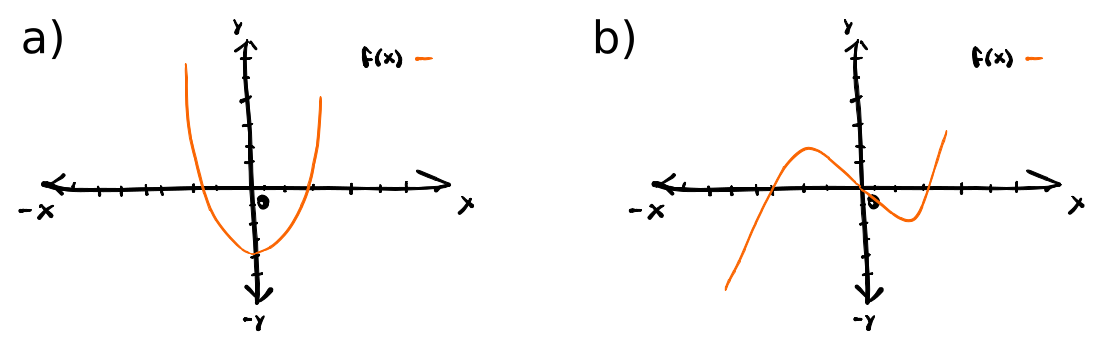
\includegraphics[scale=0.5]{parimpar.png}
\caption[Función par e impar.]{Función par e impar. a) Muestra una parábola que es una función par, es decir, los puntos ($x,y$) y (-$x,y$) son parte de la gráfica. b) Muestra una función impar, es decir, que los puntos ($x,y$) y ($-x,-y$) son parte de la gráfica.}
\label{parimparfx}
\end{figure}
\end{center}

\begin{mydef}
\textbf{Simetría.}\\

\noindent i) Una función $f$ es par si y sólo si su gráfica es simétrica respecto al $y$. \\
\noindent ii) Una función $f$ es impar si y sólo si su gráfica es simétrica respecto al origen.\\
\end{mydef}

\subsection{Transformaciones rígidas}
Este tipo de transformaciones es cualquiera que mueve la gráfica por el plano, pero no cambia la forma, es decir, son todo tipo de traslaciones de la función.\\

\begin{mydef}
\textbf{Transformaciones rígidas: Desplazamientos verticales y horizontales.} Sea $f(x)$ una función definida en los números reales y $c$ una constante real mayor que cero ($c>0$), entonces, las gráficas se someten a las siguientes traslaciones:\\

\noindent i) $y=f(x)+c$ es la gráfica desplazada verticalmente en $c$ hacia arriba.\\

\noindent ii) $y=f(x)-c$ es la gráfica desplazada verticalmente en $c$ hacia abajo.\\

\noindent iii) $y=f(x+c)$ es la gráfica desplazada horizontalmente en $c$ unidades hacia la izquierda.\\

\noindent iv) $y=f(x-c)$ es la gráfica desplazada horizontalmente en $c$ unidades hacia la derecha.\\
\end{mydef}

Se puede combinar estas traslaciones, que en el gráfico sería trasladar en \textit{diagonal} a la función y con las fórmulas de la definición anterior es $y=f(x\pm c)\pm c$.

\begin{center}
\begin{figure}[h!]
\centering
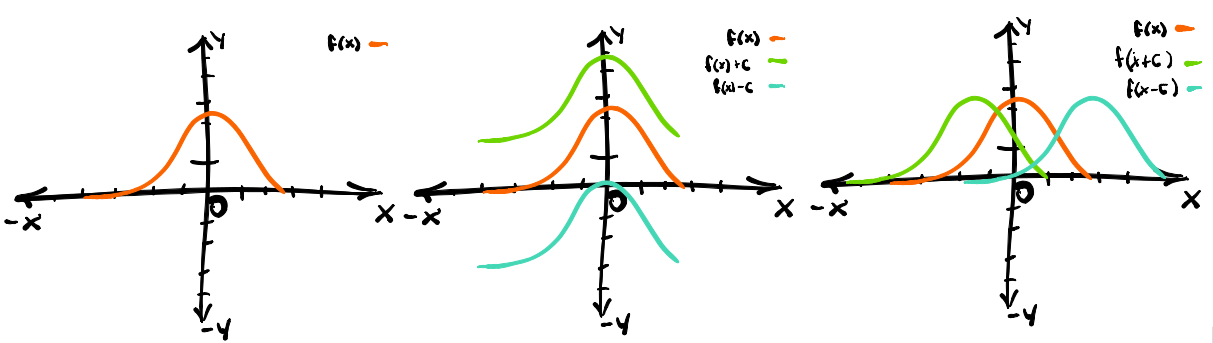
\includegraphics[scale=0.5]{trasfn.png}
\caption[Transformaciones rígidas.]{Transformaciones rígidas. a) Es la función original. b) Muestra la función original (linea naranja) y sus traslaciones verticales en $c$ unidades. c) Muestra la función original y sus respectivas traslaciones horizontales en $c$ unidades.}
\label{trasfx}
\end{figure}
\end{center}

\begin{mydef}
\textbf{Reflexiones.} Sea $f(x)$ una función definida en los números reales, entonces:

\noindent i) $y=-f(x)$ es la gráfica de $f(x)$ reflejada en el eje $x$.\\
\noindent ii) $y=f(-x)$ es la gráfica de $f(x)$ reflejada en el eje $y$. \\
\end{mydef}
%ejemplos 
\subsection{Transformaciones no rígidas}
A diferencia de la subsección anterior, ahora si se modificará la forma de la función original. Ahora, la función se puede achatar, estirar o en otros casos cambiar la pendiente.
\begin{mydef}
\textbf{Transformaciones no rígidas: Estiramientos y compresiones verticales.} Sea $f(x)$ una función definida en los números reales, entonces la gráfica de $y=c\cdot f(x)$ es:\\

\noindent i) Estirada verticalmente por un factor de $c$ unidades, si $c>1$.\\

\noindent ii) comprimida verticalmente por un factor de $c$ unidades, si $0<c<1$.\\
\end{mydef}

\begin{center}
\begin{figure}[h!]
\centering
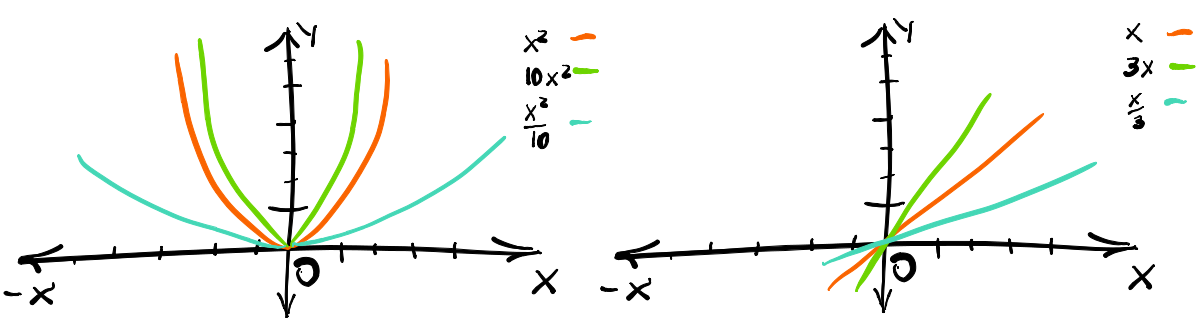
\includegraphics[scale=0.35]{deforfn.png}
\caption[Transformaciones no rígidas.]{Transformaciones no rígidas. Se ven las posibilidades de deformar la función $f(x)$ cambiando su forma, para el gráfico de la izquierda es una función cuadrática con forma $y=a_{2}x^{2}$ y el de la derecha es una función lineal de la forma $y=a_{1}x+a_{0}$. La definición de coeficientes se ve en la ecuación (\ref{polg00}).}
\label{deforfx}
\end{figure}
\end{center}

\section{Función cuadrática y lineal}
\label{fnlincua}
Anteriormente vimos a los polinomios y su forma más general (ver la ecuación  \ref{polg00}), entonces ahora veremos algunos casos particulares. Recordando la fórmula de un polinomio con un exponente $n$ que es entero y no negativo
\begin{eqnarray}
f(x)=a_{n}x^{n}+a_{n-1}x^{n-1}+\cdots +a_{2}x^{2}+a_{1}x+a_{0}
\label{polfn}
\end{eqnarray}
De (\ref{polfn}) desprenderemos tres casos. La constante es cuando $a_{0}\neq 0$, el caso lineal es cuando $a_{0},a_{1}\neq 0$ y el caso cuadrático es cuando $a_{0},a_{1}, a_{2}\neq 0$.

\begin{mydef}
\textbf{Funcionales polinomiales.} Sea $f(x)$ una función polinomial definida en los números reales, se desprenden los siguientes casos:\\

\noindent i) Si $f(x)=a$ es una función constante.\\
\noindent ii) Si $f(x)=ax+b$ es una función lineal.\\
\noindent iii) Si $f(x)=ax^{2}+bx+c$ es una función cuadrática.\\

Los coeficientes $a_{0}$, $a_{1}$ y $a_{2}$ fueron redefinidos por simplicidad, pero no se pierde generalidad.\\
\end{mydef}

\subsection{Función lineal}
Ya tuvimos una aproximación con este tipo de cuentas y lucen como el gráfico a la derecha de la figura (\ref{deforfx}). El caso más simple es cuando la recta pasa por el origen, por lo que la función luce de la forma $f(x)=ax$. El coeficiente $a$ nos da la pendiente de la recta, es decir, si $a$ negativo la recta cambia su sentido.\\

El dominio de estas funciones (y el de todas las funciones polinomiales que no son fracciones) son todos los números reales, porqué en ningún caso se indetermina la expresión.
\begin{myexample}
Muestra de algunas ecuaciones lineales:\\

\noindent i) $f(x)= x-2$ \\
\noindent ii) $f(x)=x $\\
\noindent iii) $f(x)= x+2 $\\
\noindent iv) $f(x)= -x$ \\

\begin{center}
\begin{figure}[h!]
\centering
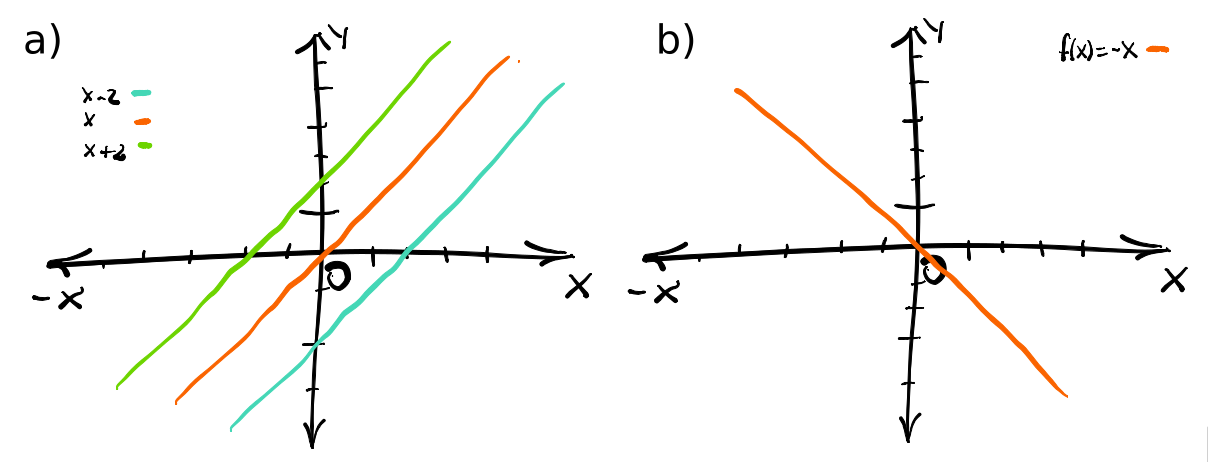
\includegraphics[scale=0.5]{linfn.png}
\caption[Funciones lineales.]{Funciones lineales. a) Ejemplo de tres funciones lineales, la recta naranja grafica la función $ii$ y las otras dos rectas son la misma función pero desplazadas (caso $i$ y $ii$). b) Gráfica de la recta $f(x)=-x$ que da muestra que el factor que acompaña a $x$ es la pendiente de la recta.} \label{linfn}
\end{figure}
\end{center}
\end{myexample}


\subsection{Función cuadrática}
Subiendo de $n$ en las funciones polinomiales nos encontramos con el caso cuadrático, usualmente llamado parábola. El caso mas simple es $f(x)=ax^{2}$, pero el caso más general tiene deformaciones y traslaciones que la dejan de la forma $f(x)=ax^{2}+bx+c$.\\
Si el coeficiente $a<0$ la parábola es un reflejo de $ax^{2}$ con $a>0$, o lo que se dice frecuentemente que \textit{apunta hacia abajo}. El coeficiente $c$ es el que desplaza horizontal o verticalmente la gráfica.\\
\newpage
\begin{myexample}
Muestra de algunas ecuaciones cuadráticas:\\

\noindent i) $f(x)= x^{2}-2$ \\
\noindent ii) $f(x)=x^{2} $\\
\noindent iii) $f(x)= x^{2}+2 $\\
\noindent iv) $f(x)= -x^{2}$ \\

\begin{center}
\begin{figure}[h!]
\centering
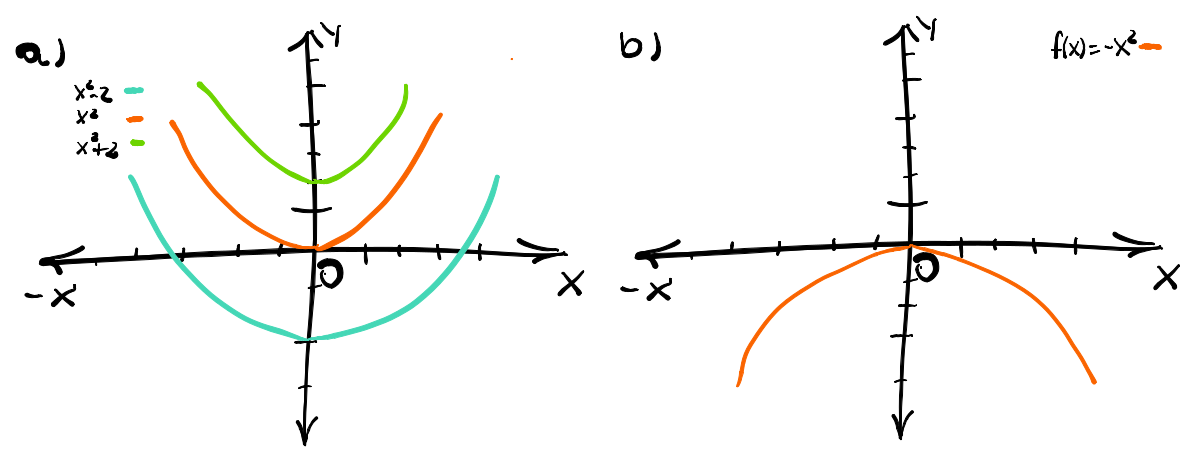
\includegraphics[scale=0.5]{cuafn.png}
\caption[Funciones cuadraticas.]{Funciones cuadráticas. a) Gráfica de funciones cuadráticas desplazadas con respecto a la función original $f(x)=x^{2}$. b) Gráfica de la función parabólica de $f(x)=-x^{2}$ que es el reflejo con respecto al eje $x$ de $x^{2}$. } \label{cuadfn}
\end{figure}
\end{center}
\end{myexample}


\subsubsection{Vértice y eje}
Los puntos que caracterizan a una parábola son el signo de $a$ para ver hacia donde crece, los posibles puntos de intersección con el eje $x$ y su vértice. La parábola puede estar apuntando hacia arriba ($a>0$) o hacia abajo ($a<0$), el punto más abajo ($a>0$) o más arriba ($a<0$) se llama vértice. Este punto marca la mitad de la parábola, que al hacer una línea en $x=h$ marca el eje de simetría. La forma matemática de obtener el vértice de una parábola cualquiera es la siguiente:\\
\begin{eqnarray}
f(x)=a(x-h)^{2}+k,\label{eqver}
\end{eqnarray}
ahora modificaremos el polinomio de segundo grado para compararlos con (\ref{eqver}).
\begin{eqnarray}
f(x)&=& ax^{2}+bx+c\nonumber\\
f(x)&=& a\left(x^{2}+\dfrac{b}{a}x \right)+c\nonumber\\
f(x)&=& a\left(x^{2}+\dfrac{b}{a}x-\dfrac{b^{2}}{4a^{2}}+\dfrac{b^{2}}{4a^{2}}  \right)+c\nonumber\\
f(x)&=& a\left(x^{2}+\dfrac{b}{a}x+\dfrac{b^{2}}{4a^{2}} \right)-\dfrac{b^{2}}{4a} +c\nonumber\\
f(x)&=& a\left(x+\dfrac{b}{2a} \right)^{2}+\dfrac{4ac-b^{2}}{4a} \label{eqver0}
\end{eqnarray}
Luego, se compara término a término entre las ecuaciones (\ref{eqver}) y (\ref{eqver0}), por lo que el vértice y el eje quedan definidos como:\\
\begin{eqnarray*}
h=\dfrac{-b}{2a}\hspace{6px}y\hspace{6px}k=\dfrac{4ac-b^{2}}{4a}
\end{eqnarray*}
En consecuencia el vértice de la parábola $(h,k)$. El punto del vértice es:
\begin{eqnarray}
\left(-\dfrac{b}{2a},f\left(-\dfrac{b}{2a} \right) \right)
\end{eqnarray}

Notar que para llegar a la ecuación (\ref{eqver0}) se realizó la operación de completar cuadrado (Para ver en detalle el completar cuadrado revisar el apéndice \ref{completarbi}). Consiste en sumar y restar un mismo termino, es decir, un cero para que quede un cuadrado de binomio de la forma $(a+b)^{2}$ más un término.  

\subsubsection{Intersección con los ejes}
Para encontrar los puntos en que la parábola pasa por los ejes utilizaremos un concepto ya visto, la soluciones de la ecuación de segundo grado. En la ecuación (\ref{raicesseg}) se ven las dos soluciones, que son justamente los dos puntos donde la parábola toca el eje $x$.\\ 
\begin{eqnarray}
x_{+}=\dfrac{-b+\sqrt{b^{2}-4ac}}{2a} \hspace{6px}y\hspace{6px}x_{-}=\dfrac{-b-\sqrt{b^{2}-4ac}}{2a}
\label{raicesseg}
\end{eqnarray}
Los puntos $x_{+}$ y $x_{-}$ son los que muestran las intersecciones con el eje $x$.

\begin{myexample}
Encontrar las intersecciones y el vértice de la siguiente función:
\begin{eqnarray*}
f(x)&=& x^{2}+2x-3\\
f(x)&=& (x+1)(x-3)\\
x=-1 &y& x=3\\
(-1,0) &y& (3,0)\\
\end{eqnarray*}
Para el vértice se debe completar cuadrados para igualar $f(x)$ con la ecuación (\ref{eqver}).
\begin{eqnarray*}
f(x)&=& x^{2}-2x-3\\
f(x)&=& x^{2}-2x+1-1-3\\
f(x)&=& (x^{2}-2x+1)-4\\
f(x)&=& (x-1)^{2}-4\\
f(x)&=& a(x-h)^{2}+k\\
\end{eqnarray*}
Al comparar los términos se obtiene que el vértice de la parábola está en el punto $(1,-4)$.
\end{myexample}

\section{Funciones crecientes y decrecientes}
\label{funcrede}
Hemos visto en las figuras (\ref{deforfx}), (\ref{linfn}) y (\ref{cuadfn}) un comportamiento de las funciones que aumentan y disminuyen por tramos. Cuando la función se mantiene en una tendencia de crecer o decrecer se clasifican en los siguientes casos:
\begin{mydef}
\textbf{Funciones crecientes y decrecientes.} Sea $f(x)$ una función real que está definida en un intervalo con extremos $x_{1}$ y $x_{2}$, que son dos números cualesquiera tales que $x_{1}<x_{2}$. Entonces, se cumple lo siguiente:\\

\noindent i) La función $f(x)$ es creciente en el intervalo si, $f(x_{1})<f(x_{2})$. \\
\noindent ii) La función $f(x)$ es decreciente en el intervalo si, $f(x_{1})>f(x_{2})$.  \\

\begin{center}
\begin{figure}[h!]
\centering
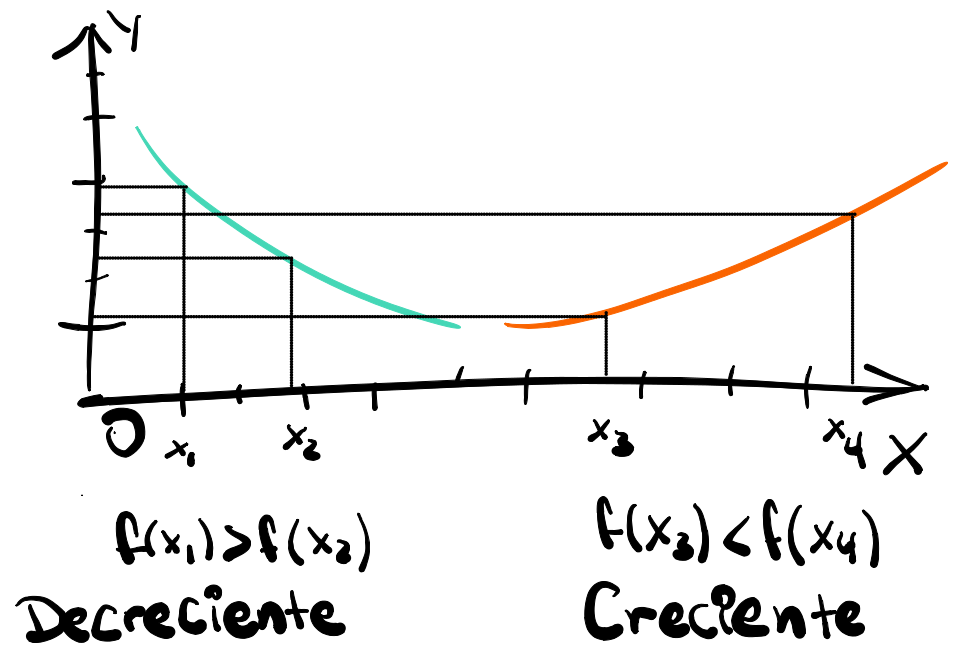
\includegraphics[scale=0.30]{credrefn.png}
\caption[Funciones crecientes y decrecientes.]{Funciones crecientes y decrecientes. .} \label{credrefn}
\end{figure}
\end{center}
\end{mydef}

Esta clasificación es una primera herramienta para saber como se comporta la función y consiste en seleccionar dos elementos del dominio para ver la respectiva imagen. Se debe considerar que una herramienta más poderosa se verán más adelante en el capítulo de calculo infinitesimal.

\begin{myexample}
Sean las funciones $f(x)=x^{2}$ y $g(x)=-x^{2}$ definida en los números reales. Seleccione dos elementos del dominio y mencione si es creciente o decreciente.\\

i) $f(x)=x^{2}$:\\
\begin{eqnarray*}
f(x_{1})&=& f(x_{1}=3)=f(3)=3^{2}=9\\
f(x_{2})&=& f(x_{2}=4)=f(4)=4^{2}=16
\end{eqnarray*}
$x_{2}>x_{1}$, por lo que $f(x)$ es una función creciente en este intervalo. \\

i) $g(x)=-x^{2}$:\\
\begin{eqnarray*}
f(x_{1})&=& f(x_{1}=3)=f(3)=-3^{2}=-9\\
f(x_{2})&=& f(x_{2}=4)=f(4)=-4^{2}=-16
\end{eqnarray*}
$x_{2}<x_{1}$, por lo que $g(x)$ es una función decreciente en este intervalo. \\
\end{myexample}
Si los valores coinciden para ambos $x$, entonces es una función constante.
\newpage
\section{Funciones por partes}
Como el nombre lo dice, es una función que según el tramo del dominio que uno seleccione va a tener una función diferente. El primer acercamiento es el valor absoluto, que en su versión mas simple son dos rectas con pendientes opuestas (ver la definición \ref{absdef}).\\

\begin{myexample}
\textbf{Función por tramos}. Cantidades de medicina (mg) contra la alergia según la edad del paciente (años):\\
%\begin{center}
%\begin{table}[h!]
%\centering
%\begin{tabular}{|c|c|}
%\hline
%Bajo $6$ años de edad &Preguntar al Doctor \\
%\hline
%De $6$ a $12$ años& $12,5$ a $25$ $mg$ \\
%\hline
%De $12$ años hacia arriba & $25$ a $50$ $mg$\\
%\hline
%\end{tabular}
%\caption[Tabla de medicina anti alergia según la edad.]{Tabla de medicina anti alergia según la edad.}
%\end{table}
%\end{center}
%Esta tabla se puede pasar a una función por tramos 

$$ f(x)= \left\{\begin{array}{ll}
Preguntar\hspace{3px} al\hspace{3px} doctor&,\hspace{2px} si\hspace{6px}0\leq x< 6\\
\dfrac{6x}{12,5}+19,24 &,\hspace{2px} si \hspace{6px}  6\leq x< 12\\ 
\dfrac{87x}{25}-16,76 &,\hspace{2px} si \hspace{6px} x \geq12
\end{array} \hspace{6px} \right.$$
El dominio de la función es rango etario que se considere (el x), mientras que la imagen son los miligramos de medicamentos.
\end{myexample}

\begin{myexample}
Se da un modelo simple\cite{Cancer} para ver si hay o no presencia de un tumor. Sea $M_{1}$, $M_{2},...,$ $M_{n}$ denota la alteración genética de interés. Esta alteración puede ser un punto de mutación, ganancia o perdida de una región cromosómica u otro evento genético. $N$ independientes especímenes (``tumores'') son obtenidos y la presencia o ausencia de la alteración de interés es guardad como un vector binario\footnote{Solo tiene dos resultados, en este caso es $0$ o $1$.} $x_{j}=\{x_{j1},x_{j2},...,x_{jn}\}$, donde: \\

	\begin{eqnarray*}
 x_{jl}= \left\{\begin{array}{ll}
0&,\hspace{4px} si\hspace{3px}en\hspace{3px}el\hspace{3px}j-esimo\hspace{3px}hay \hspace{3px}ausencia\hspace{3px}de\hspace{3px}alteraci\acute{o}n\hspace{3px}M_{l}\\
1 &,\hspace{4px} si\hspace{3px}en\hspace{3px}el\hspace{3px}j-esimo\hspace{3px}hay \hspace{3px}presencia\hspace{3px}de\hspace{3px}alteraci\acute{o}n\hspace{3px}M_{l}\\ 
				\end{array} \hspace{6px} \right.
	\end{eqnarray*}
	
Si tenemos por ejemplo el vector $x_{1}=\{x_{11},x_{12},..,x_{1n}\}$, ahora se debe calcular cada elemento del vector con la función por partes, por ejemplo si tomamos el primer elemento $x_{11}$.\\

	\begin{eqnarray*}
 x_{11}= \left\{\begin{array}{ll}
0&,\hspace{4px} si\hspace{3px}en\hspace{3px}el\hspace{3px}j-esimo\hspace{3px}hay \hspace{3px}ausencia\hspace{3px}de\hspace{3px}alteraci\acute{o}n\hspace{3px}M_{1}\\
1 &,\hspace{4px} si\hspace{3px}en\hspace{3px}el\hspace{3px}j-esimo\hspace{3px}hay \hspace{3px}presencia\hspace{3px}de\hspace{3px}alteraci\acute{o}n\hspace{3px}M_{1}\\ 
				\end{array} \hspace{6px} \right.
	\end{eqnarray*}
	
El dato de $0$ o $1$ estará dado por los datos recolectados de la muestra $M_{1}$, entonces una ejemplo del vector binario es $x_{j}=\{x_{j1},x_{j2},...,x_{jn}\}=\{0,1,0,...,0\}$.
\end{myexample}


\begin{myexample}
Graficar la siguiente función por tramos:
\begin{eqnarray*}
 f(x)= \left\{\begin{array}{ll}
-1&, x< 0\\
0 &, x=0\\ 
x+1 &, x>0 \\
\end{array} \hspace{6px} \right.
\end{eqnarray*}

\begin{center}
\begin{figure}[h!]
\centering
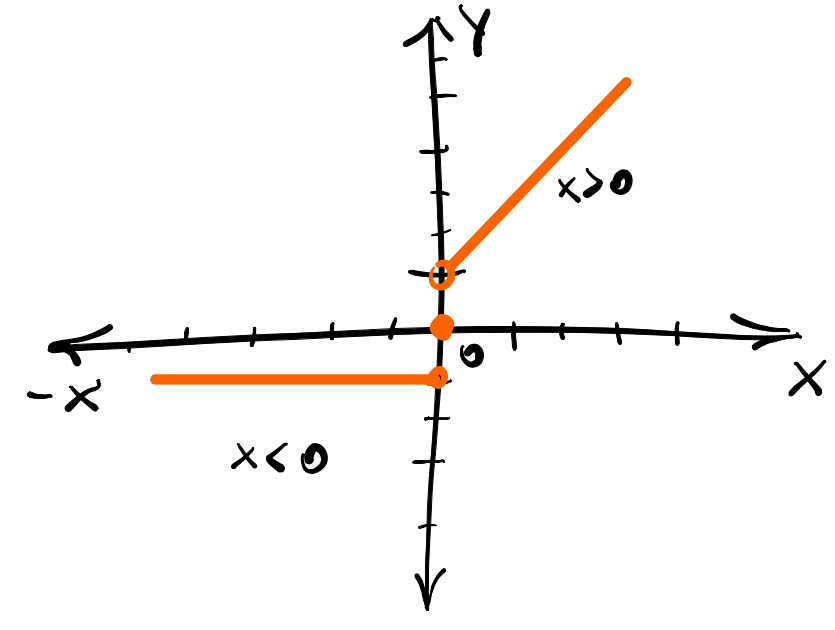
\includegraphics[scale=0.3]{partefn.png}
\caption[Función por partes.]{Función por partes. Son tres funciones, la primera es una función constante, la segunda un punto y la tercera es una recta. Notar que los extremos de la primera y tercera función consideran los extremos (por eso los círculos sin pintar). } \label{partefn}
\end{figure}
\end{center}
\end{myexample}
La lógica de las funciones por partes es igual, pero veremos un caso particular por su uso cotidiano. La función es una unión de funciones constantes, con dominio continuo si se unen los dominios de las partes, usualmente se llama \textit{función máximo entero}.
\begin{eqnarray*}
 f(x)= \left\{\begin{array}{ll}
 \vdots \\
-2&, -2\leq x< -1\\
-1&, -1\leq x<0\\ 
0 &, 0\leq x < 1\\
1&, 1\leq x <2\\
\vdots
\end{array} \hspace{6px} \right.
\end{eqnarray*}
%escalerafn.png

\begin{center}
\begin{figure}[h!]
\centering
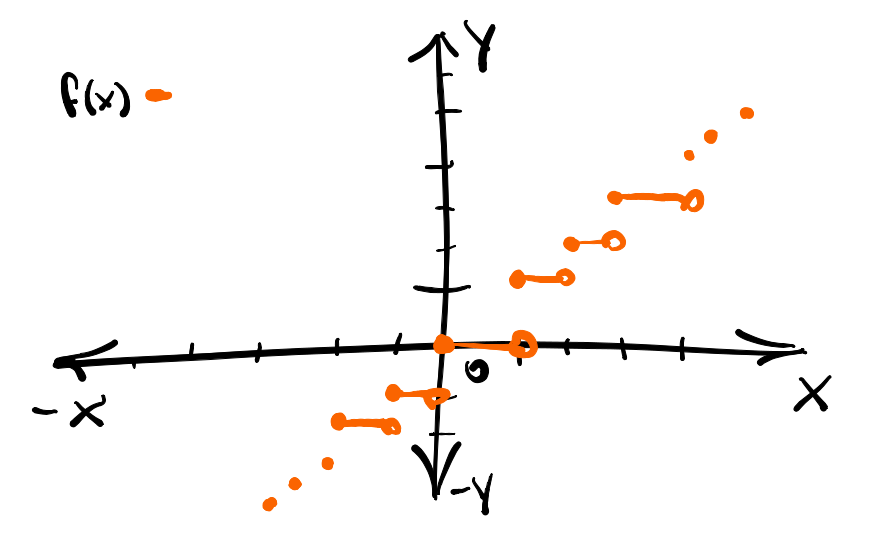
\includegraphics[scale=0.30]{escalerafn.png}
\caption[Función máximo entero.]{Función máximo entero.  } \label{escalerafn}
\end{figure}
\end{center}

La imagen de la función es discreta, es decir, tomar ciertos valores y no es un \textit{continuo} de valores. 
\newpage
\subsection{Dominio de una función por partes}

Al momento de analizar el dominio completo de la función por partes, se debe ver la definición de la misma. Si se ve el lado derecho, se encuentran las expresiones de las funciones y al lado izquierdo los intervalos en los cuales se defines las funciones, justamente son el dominio de cada función. Entonces, el dominio de la función por partes es la unión de cada uno de los dominios de la funciones que lo conforman.\\

\begin{myexample}
Encontrar el dominio de siguiente función por partes:
\begin{eqnarray*}
 f(x)= \left\{\begin{array}{ll}
f_{1}(x)&, x< 0\\
f_{2}(x) &, x=0\\ 
f_{3}(x) &, x>0 \\
\end{array} \hspace{6px} \right.
\end{eqnarray*}
$Dom(f(x))=Dom(f_{1}(x))\cup Dom(f_{2}(x))\cup Dom(f_{3}(x))=\mathbb{R}$
\end{myexample}
En el ejemplo anterior se ve que el dominio son todos los números reales, ya que entre los tres dominios completan el intervalo $]-\infty,\infty[$. En el caso en que algún punto o intervalo no sea considerado aparecen los tramos en que la función no está definida.

\begin{myexample}
Encontrar el dominio de siguiente función por partes:
\begin{eqnarray*}
 g(x)= \left\{\begin{array}{ll}
g_{1}(x)&, -5<x<1\\
g_{2}(x) &, 1\leq x\leq 10\\ 
g_{3}(x) &, 15<x<20 \\
\end{array} \hspace{6px} \right.
\end{eqnarray*}

\begin{eqnarray*}
Dom(g(x))&=& Dom(g_{1}(x))\cup Dom(g_{2}(x))\cup Dom(g_{3}(x))\nonumber\\
&=&]-5,1[\cup [1,10]\cup ]15,20[\\
&=&]-5,10]\cup ]15,20[\\
\end{eqnarray*}
\end{myexample}
Para este caso se ve, en la definición y en el resultado del dominio, que la función tiene tramos no definidos. Específicamente, los intervalos $]-\infty,-5]$, $]10,15]$ y $[20,\infty[$ no son parte del dominio.

\section{Combinación de funciones}
Luego de ver las funciones por partes, sigue la opción de combinar funciones, que en estricto rigor ya lo hemos visto cuando sumamos, restamos o dividimos polinomios. Las operaciones formales que se pueden hacer al momento de combinar funciones son: \\
\begin{mydef}
\textbf{Combinación de funciones.} Sea $f(x)$ y $g(x)$ dos funciones definidas en los números reales, entonces las operaciones de suma ($+$), resta ($-$), división ($\slash$) y la multiplicación ($\cdot$) se define de la siguiente manera:\\

\noindent i) $(f+g)(x)=f(x)+g(x)$.\\
\noindent ii) $(f-g)(x)=f(x)-g(x)$.\\
\noindent iii) $(f\cdot g)(x)=f(x)\cdot g(x)$.\\
\noindent iv) $\left(\dfrac{f}{g} \right)(x)=\dfrac{f(x)}{g(x)}$, siempre que $g(x)\neq 0$.\\
\end{mydef}

\begin{myexample}
Escribir la función resultante de las cuatro operaciones con las funciones $f(x)=x^{2}-1$ y $g(x)=x+1$:\\

\noindent i)$f(x)+g(x)=x^{2}+x$.\\
\noindent ii) $f(x)-g(x)=x^{2}-x-2$.\\
\noindent iii) $f(x)\cdot g(x)=(x^{2}-1)(x+1)=x^{2}(x+1)-(x+1)=x^{3}+x^{2}-x-1$.\\
\noindent iv) $\dfrac{f(x)}{g(x)}=\dfrac{x^{2}-1}{x+1}=\dfrac{(x+1)(x-1)}{x+1}=x-1$.\\
\end{myexample}

\subsection{Dominio de una función combinada}
Es importante que por más combinaciones que se hagan entre dos o más funciones sigan estando definidas en los números reales, suena obvio, pero hay verificarlo. El dominio que tiene una función combinada es el conjunto más grande que tiene en común todas las funciones, entonces es la intersección del dominio de las funciones. Para el caso de la división se suma la condición que la expresión del denominador debe ser diferente de cero.\\
 Supongamos el ejemplo que tenemos dos funciones $f_{1}(x)$ y $f_{2}(x)$ con su conjunto dominio $X_{1}$ y $X_{2}$ respectivamente. Entonces, el dominio de la función combinada es: \\
 
 \noindent i) El dominio para las operaciones de suma, resta y y multiplicación es $X_{1}\cap X_{2}$.\\
 
  \noindent ii) El dominio para las operacion de división es $\{x|x\in  X_{1}\cap X_{2}, g(x)\neq 0\}$.\\
  
\begin{myexample}
Sea $f(x)=\sqrt{x-3}$ y $g(x)=\sqrt{x+4}$ dos funciones definidas en los números reales, calcule el dominio de la función combinada $f(x)/g(x)$.\\

\textit{Sol:} Primero sabemos que las funciones de raíz cuadrada estén definidas en los números reales y deben ser mayor o igual que cero ($\geq 0$). Además, la función del denominador debe cumplir que $g(x)\neq 0$.\\
%Agregar definición con cuantificadores
\begin{eqnarray*}
h(x)=\dfrac{f(x)}{g(x)}&=&\dfrac{\sqrt{x-3}}{\sqrt{x+4}}\\
Dom(f(x))&\cap &Dom(g(x)), g(x)\neq 0\\
x-3\geq 0 &\cap &x+4>0\\
x\geq +3 &\cap &x>-4 \\
\left[3,+\infty \right] &\cap & \left]-4,+\infty \right[\\
Dom\left(\dfrac{f(x)}{g(x)} \right) &=&\left[3,+\infty \right] 
\end{eqnarray*}
Notar que la condición del denominador sea diferente de cero se cumplió al pasar de $\geq$ a $>$.
\end{myexample}

\section{Composición de funciones}
Al principio de esta sección se mencionó que dentro del paréntesis de la función ($f()$) va la incógnita, por ende lo que se reemplaza en este caso es la función $f()$. En esta sección veremos que ocurre cuando dentro de la función hay otra función, como por ejemplo $f(g(x))$.\\

\begin{mydef}
\textbf{Composición de funciones.} Sea $f(x)$ y $g(x)$ dos funciones definidas en los números reales. La composición de ambas funciones se escribe de la siguiente manera:\\
\begin{eqnarray*}
(f\circ g)(x)&=& f(g(x)) \\
(g\circ f)(x)&=&g(f(x)) \\
\end{eqnarray*}
\end{mydef}

\begin{myexample}
Sea $f(x)=x^{2} +x$ y $g(x)=x+5$ dos funciones definidas en los números reales, calcular las funciones compuestas $f(g(x))$ y $g(f(x))$.\\
\begin{eqnarray*}
f(g(x))&=& f(x+5)= (g(x))^{2}+(g(x))=(x+5)^{2}+(x+5)\\
&=& x^{2}+10x+25+x+5\\
&=&x^{2}+11x+30.
\end{eqnarray*}
\begin{eqnarray*}
g(f(x))&=& g(x^{2}+x)=g(x)+5=x^{2}+x+5 \\
\end{eqnarray*}
\end{myexample}


\subsection{Dominio de una función compuesta}
El dominio de la función compuesta es el conjunto formado por los números que están en el dominio de $g(x)$, tales que $g(x)$ esté en el dominio de $f(x)$. En otras palabras, son los números que están en g(x) y que además no indeterminan $f(x)$. La definición del dominio de una función compuesta por $f(x)$ y $g(x)$ es:
\begin{eqnarray}
Dom\left(f(g(x)) \right)=\{x\in Dom(g(x))\wedge g(x)\in Dom(f(x))\}\\
Dom\left(g(f(x)) \right)=\{x\in Dom(f(x))\wedge f(x)\in Dom(g(x))\}
\end{eqnarray}

\begin{myexample}
Sea $f(x)=x/(x+2)$ y $g(x)=1/(x-1)$ dos funciones definidas en los números reales. Calcular el dominio de la función compuesta $f(g(x))$.

\begin{eqnarray*}
Dom(f(g(x)))&=& x\in Dom(g(x)) \wedge g(x)\in Dom(f(x))\\
&=& x\neq 1 \wedge \dfrac{1}{x-1}\neq -2\\
&=& x\neq 1 \wedge x\neq\dfrac{1}{2}\\
&=& \mathbb{R}-\{1\} \cap \mathbb{R}-\biggl\{\dfrac{1}{2}\biggl\}\\
&=&\mathbb{R}-\biggl\{ 1,\dfrac{1}{2}\biggl\}
\end{eqnarray*}
\end{myexample}

\begin{myexample}
Sea $f(x)=\sqrt{x}$ y $g(x)=x-2$. Calcular el dominio de $f(g(x))$:\\
\begin{eqnarray*}
Dom(f(g(x)))&=& Dom(f(x-2))\\
&=& Dom(\sqrt{x-2})\\
&=& \sqrt{x-2}\\
&=& x-2\geq 0\\
&=& x\geq 2\\
Dom(f(g(x)))&=& [2,+\infty [ \\
\end{eqnarray*}
\end{myexample}

\section{Cociente de diferencias}
\label{cuociente0}
Ahora, veremos una aplicación de la composición de funciones. Suponga que tomamos dos puntos del gráfico de una función ¿Cuán cerca están estos puntos? Tanto como uno quiera. Definiremos la distancia entre los dos puntos con la variable $h$, que repito, es muy pero muy pequeña. \\ Al conocer dos puntos de una función se abre el abanico de opciones para calcular. Una de ellas es trazar una recta entre los puntos y calcular la pendiente de dicha recta. Recordando la fórmula de la pendiente de una recta:\\ 

\begin{eqnarray}
m = \dfrac{y_{2}-y_{1}}{x_{2}-x_{1}}
\end{eqnarray}
Donde $x_{i}$ y $y_{i}$ son los valores de dos puntos $(x_{1},y_{2})$ y $(x_{2},y_{2})$ en un plano cartesiano. Si hacemos lo mismo pero ahora los puntos son $(x,f(x))$ y $(x+h,f(x+h))$, la pendiente es:\\
\begin{eqnarray}
m&=&\dfrac{f(x+h)-f(x)}{(x+h)-x}\nonumber \\
m&=&\dfrac{f(x+h)-f(x)}{h}
\label{dif}
\end{eqnarray} 
La ecuación (\ref{dif}) es el primer acercamiento al cálculo infinitesimal, donde la variable $h$ además de ser pequeño representa el \textit{cambio} que sufre la función.

\begin{myexample}
Calcular el cociente de diferencias de $f(x)=x^{2}+2$.\\

\noindent Sol: Primero se debe calcular la función compuesta $f(x+h)$.
\begin{eqnarray*}
f(x+h)&=&(x+h)^{2}+2 \\
&=&x^{2}+2xh+h^{2}+2\\
\end{eqnarray*}
Ahora, reemplazamos en la ecuación (\ref{dif}):
\begin{eqnarray*}
m&=&\dfrac{f(x+h)-f(x)}{h}\\
&=&\dfrac{x^{2}+2xh+h^{2}+2-(x^{2}+2)}{h}\\
&=&\dfrac{2xh+h^{2}}{h}\\
&=&\dfrac{h(2x+h)}{h}\\
&=&2x+h,\hspace*{15px} h\approx 0\\
&=&2x \\
\end{eqnarray*}
Entonces el cocientes de diferencias de $f(x)$ es $2x$, más adelante veremos que este cociente es la \textbf{derivada} de $f(x)$ y se puede denotar como $f'(x)$.
\end{myexample}

\begin{center}
\begin{figure}[h!]
\centering
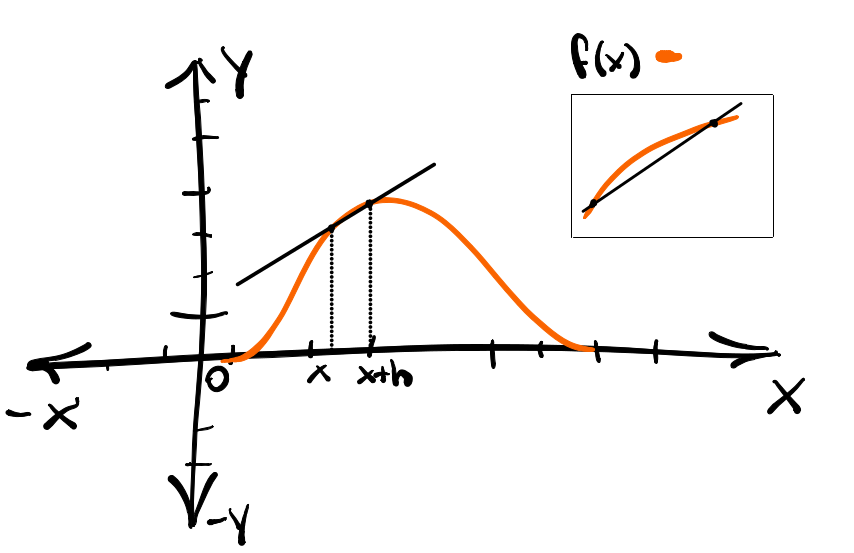
\includegraphics[scale=0.35]{cocientefn.png}
\caption[Cociente de diferencia.]{Cociente de diferencia. La línea naranja continua representa la función, la línea negra continua representa la recta de los puntos y las líneas punteadas muestran la diferencia entre los puntos (la distancia es representada por $h$). El gráfico insertado amplía la función y la recta, donde para los dos puntos hay una distancia $h$.} \label{cocifn}
\end{figure}
\end{center}
\section{Funciones inversas}
En un principio, vimos en (\ref{fn00}) que las funciones son una correspondencia entre un dominio $X$ y una imagen $Y$. Siempre a un elemento $x_{i}$ del dominio se le asocia un elemento $y_{i}$ de la imagen y por más que haya casos en que hay más de un elemento del dominio para un mismo $y_{i}$ (por ejemplo las funciones del tipo $x^{2}$), las funciones que por cada elemento del dominio tienen un solo elemento de la imagen se llaman funciones uno a uno.

\begin{mydef}
\textbf{Función uno a uno.} Sea una función $f(x)$ definida en los números reales, es uno a uno o biunívoca si cada número en el rango de $f(x)$ está asociado con exactamente con \textbf{un} número en su dominio $X$.  
\end{mydef}

La forma \textit{gráfica} de ver si una función es uno a uno es trazar una línea horizontalmente, si la línea toca dos puntos, entonces no es una función biunívoca, en caso contrario si lo es.\\
Al momento definir este tipo de funciones, se puede hacer en función de los elementos de dominio.

\begin{mydef}
\textbf{Función uno a uno.} Una función es uno a uno si y solo si $f(x_{1})=f(x_{2})$ implica que $x_{1}=x_{2}$ para toda $x_{1}$ y $x_{2}$ en el dominio de f.
\end{mydef}

%%%%%
\begin{center}
\begin{figure}[h!]
\centering
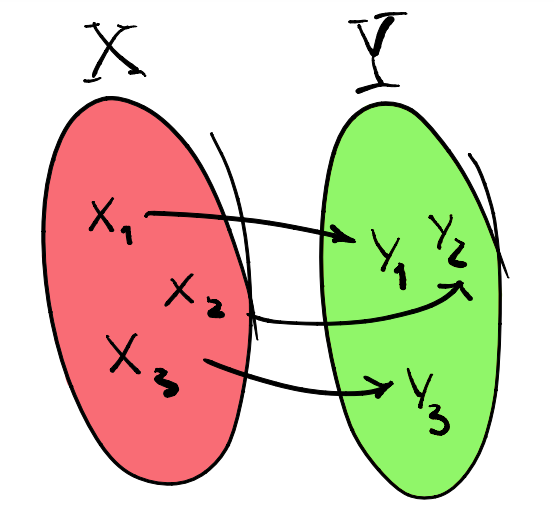
\includegraphics[scale=0.4]{unoaunofn.png}
\caption[Función uno a uno.]{Función uno a uno. Los óvalos rojos y verde representan el dominio e imagen de la función $f(x)$. Las flechas muestran que cada elemento $x_{i}$ $(i=1,2,3)$ del dominio tiene un elemento $y_{i}$ $(i=1,2,3)$ de la imagen.} \label{unafn}
\end{figure}
\end{center}
\begin{myexample}
Sea $f(x)=x+1$, comprobar si es una función uno a uno.
\begin{eqnarray*}
x_{1}+1&=&x_{2}+1 \hspace{10px} \slash -1 \\
x_{1}&=&x_{2}
\end{eqnarray*}
Como $x_{1}=x_{2}$ implica que $f(x_{1})=f(x_{2})$, por lo tanto $f(x)$ es una función uno a uno.
\end{myexample}

\begin{myexample}
Sea $f(x)=x^{2}+1$, comprobar si es una función uno a uno.

\begin{eqnarray*}
x_{1}^{2}+1&=&x_{2}^{2}+1 \hspace{10px} \slash -1 \\
x_{1}^{2}&=&x_{2}^{2}  \hspace{10px} \slash \sqrt{•}\\
\sqrt{x_{1}^{2}}&=&\sqrt{x_{2}^{2}}\\
|x_{1}|&=&|x_{2}|\\
\end{eqnarray*}
Como ambos $x_{i}$ están con valor absoluto, puede dar el caso de que $x_{1}=-x_{2}$ o $-x_{1}=x_{2}$, por lo tanto no se cumplen las condiciones de una función biunívoca. Entonces, como $x_{1}\neq x_{2}$ implica que $f(x_{1})\neq f(x_{2})$ y $f(x)$ no es una función uno a uno.
\end{myexample}

Si imaginamos que el tomar un elemento $x_{1}$ del dominio $X$ de la función $f(x)$ es un \textit{camino de ida} y que además esta función es uno a uno, podemos hacer el \textit{camino de vuelta} para pasar de un elemento de la imagen $y_{i}$ al elemento del dominio $x_{i}$. Esto implica aplicar una función (desconocida hasta el momento) que pase los elementos de la imagen al dominio de la función, esa función se llama función inversa.

\begin{mydef}
\textbf{Función inversa.} Sea f(x) una función uno a uno, con dominio $X$ e Imagen $Y$. La inversa de f(x) es la función denotada por $f^{-1}$, cuyo dominio es $Y$ e imagen $X$.

\noindent i) $f(f^{-1}(x))=x$ para toda $x$ en $Y$.\\
\noindent ii) $f^{-1}(f(x))=y$ para toda $y$ en $X$.\\
\end{mydef}

\begin{mydef}
\textbf{Propiedades de las funciones inversas.} Sea $f(x)$ una función en los números reales.\\

\noindent i) $Dom(f^{-1}(x))=Img(f(x))$. \\

\noindent ii) $Dom(f(x))=Img(f^{-1}(x))$. \\

\noindent iii) $y=f(x)$ equivale a $x=f^{-1}(y)$. \\

\noindent iv) La función inversa $f^{-1}$ es uno a uno. \\

\noindent v) La función inversa de $f(x)$ es $f^{-1}(x)$, entonces $f^{-1}(f^{-1}(x))=f(x)$ . \\

\noindent vi) La inversa de $f(x)$ es única. \\
\label{propinv}
\end{mydef}

\begin{center}
\begin{figure}[h!]
\centering
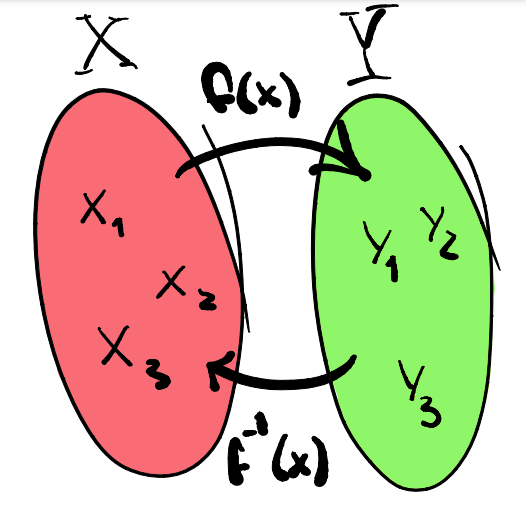
\includegraphics[scale=0.4]{inversafn.png}
\caption[Función inversa.]{Función inversa. Las flechas negras muestran que la función $f(x)$ va desde el dominio a la imagen y $f^{-1}$ va desde la imagen al dominio.} \label{inversafn}
\end{figure}
\end{center}

\begin{myexample}
Sea $f(x)=$, determinar la función inversa de $f(x)$. \\

\noindent Sol: En términos generales, se cambian los $'x'$ de la expresión por $f^{-1}(x)$ o por $'y'$ y luego se despeja dicha variable cambiada.\\
\begin{eqnarray*}
f(x)&=&\sqrt{x+3} \\
y=\sqrt{x+3}& \longrightarrow &x=\sqrt{y+3} \\
x&=&\sqrt{y+3}\\
x^{2}&=&y+3 \\
x^{2}-3 &=&y \hspace*{8px}\longleftarrow inversa\\
\end{eqnarray*}
El $Dom(f^{-1}(x))$ son todos los números reales, que a su vez es la imagen de $f(x)$.
\end{myexample}

\subsection{Gráficas de la función inversa}
En las propiedades vistas en las definiciones (\ref{propinv}) y en la figura (\ref{inversafn}) se ve que la función y su inversa son \textit{opuestas}. En términos gráficos, si los puntos $(x_{i},y_{i})$ del plano pertenecen a la función $f(x)$, los puntos de la inversa $f^{-1}(x)$ son ($y_{i},x_{i}$). Esto es que la representación de la función inversa  es una reflexión de la función original. \\
 


\begin{center}
\begin{figure}[h!]
\centering
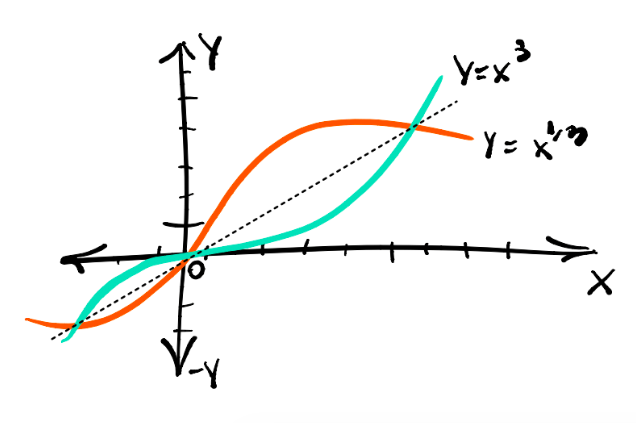
\includegraphics[scale=0.4]{invergrfn.png}
\caption[Grafico de una función inversa.]{Grafico de una función inversa. La función inversa es la reflexión con respecto al eje de simetría (representado por la linea negra punteada).} \label{Graficofnin}
\end{figure}
\end{center}

%\section{Problemas con enunciado}
%En esta sección juntaremos los conceptos para acercarlos a problemas con enunciado. Usualmente, como veremos ahora y durante este curso en general son situaciones ideales, es decir, no consideramos todas variables o son situaciones ficticias para ejercitar los tópicos. 
%
%%inversa,cociente de diferencia, fn combinadas, función escalón,interseccion con los ejes, transformaciones y deformaciones, funcion par e impar
%Resolver los siguientes problemas:\\
%
%\noindent 1) El consumo de mascarillas en el año 2016 tuvo la forma $5x+60$ y en el 2020 fue $10x-90$. Si $x$ representa los días del año ($x=1,2,3,...,365$), responda las siguientes preguntas:\\
%
%\noindent 1.a) ¿ Qué función cruza el eje $y$ en su parte positiva?
%\noindent \textit{Sol:} $f(x)=5x+60$ \\
%
%\noindent 1.b) ¿ Qué función cruza el eje $x$ en su parte positiva? 
%\noindent \textit{Sol:} $f(x)=10x-90$\\
%
%\noindent 1.c) ¿ En que año se utilizaron más mascarillas en diciembre?\\
%\noindent \textit{Sol:} Una pista se puede deducir por la pendiente de la función del año 2020, que es mayor, entonces ese es el año de mayor uso en diciembre. Lo segundo es reemplazar un número de $x$ que equivaldría a estar en diciembre \\
%\begin{eqnarray*}
%5x+60 \hspace{8px} &vs& \hspace{8px} 10x-90 \\
%5(360)+60 \hspace{8px} &vs& \hspace{8px} 10(360)-90 \\
%1860 \hspace{8px} &< & \hspace{8px} 3510 
%\end{eqnarray*}
%Se concluye que en el año 2020 se utilizaron mas mascarillas.\\
%
%\noindent 1.d) ¿ En que día del año se ocuparon el mismo número de mascarillas?
%
%\noindent \textit{Sol:} Si se ocuparon el mismo número, nos dice que ambas rectas tuvieron la misma imagen (número de mascarillas). Entonces, se deben interceptar ambas ecuaciones lineales. \\
%\begin{eqnarray*}
%5x+60  &=&  10x-90 \\
%90+60  &=&  10x-5x\\
%150  &=&  5x\\
%x  &=&  30
%\end{eqnarray*}
%
%\begin{center}
%\begin{figure}[h!]
%\centering
%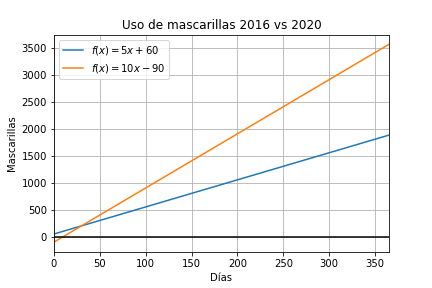
\includegraphics[scale=0.8]{mascarillas.png}
%\caption{Gráfica de las rectas del problema 1.} \label{prob1}
%\end{figure}
%\end{center}

\section{Funciones polinomiales}
En la sección (\ref{fnlincua}) se vio desde la función constante ($ax^{0}$) hasta la función cuadrática ($ax^{2}$), pero este tipo de funciones son parte de un conjunto más grande, las polinomiales. Ahora entraremos en detalles de como graficar este tipo de funciones. Recordar la ecuación (\ref{polfn}), donde el exponente es un número entero no negativo y en caso de que $n$ no cumpla estas condiciones, la función no es polinomial (Ejemplo: $x^{-1}$ o $x^{1/2}$).

Cuando hablamos de la función cuadrática tenemos en mente el $x^{2}$, de la misma manera pasa con el cúbico y su representación $x^{3}$. Cuando el exponente es mayor se le llama $n-$ésimo considerando el exponente mayor como nombre del polinomio (Ejemplo: $x^{8}+4$ polinomio de octavo orden). 

\begin{mydef}
\textbf{Funciones polinomiales.} Sea $f(x)$ una función polinomial definida en los números reales, se desprenden los siguientes casos:\\

\noindent i) Si $f(x)=a_{0}$ es una función polinomial constante.\\
\noindent ii) Si $f(x)=a_{1}x+a_{0}$ es una función polinomial lineal.\\
\noindent iii) Si $f(x)=a_{2}x^{2}+a_{1}x+a_{0}$ es una función polinomial cuadrática.\\
\noindent iv) Si $f(x)=a_{3}x^{3}+a_{2}x^{2}+a_{1}x+a_{0}$ es una función polinomial cúbica.\\
\noindent v) Si $f(x)=a_{n}x^{n}+a_{n-1}x^{n-1}+\cdots+a_{0}x^{0}$ es una función polinomial $n-$ésima.
\end{mydef}

En (\ref{linfn}) y (\ref{cuadfn}) se muestra la gráfica de las funciones lineales y cuadrática respectivamente, pero es más difícil a simple vista dilucidar las gráficas de órdenes mayores. Por lo mismo, hay que tener en consideración conceptos anteriores como traslaciones, deformaciones, simetrías o intersecciones con los ejes. \\

Lo más simple es partir por el caso en que la función es un solo término de la forma $x^{n}$, aquí se puede tener el caso en que $n$ es par o impar. \\

\begin{center}
\begin{figure}[h!]
\centering
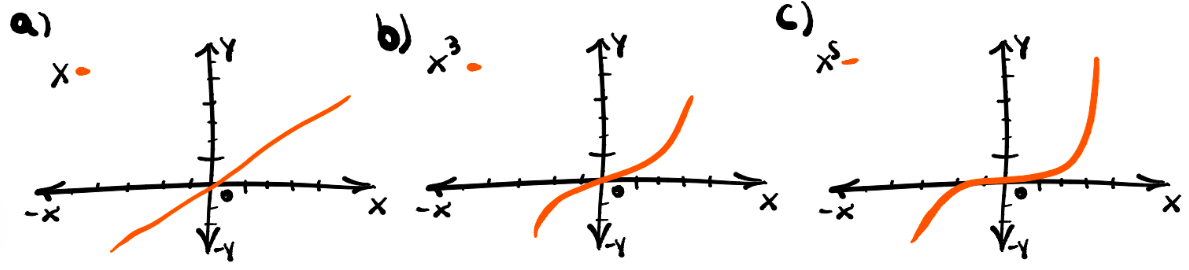
\includegraphics[scale=0.5]{fnimpares.png}
\caption[Ejemplo funciones impares.]{Ejemplo funciones impares. a) Es la función lineal y en los casos b) y c) se ve como se va aplanando la región que pasa por el origen del plano a medida que aumenta el $n$ de $x^{n}$.} \label{fnimp}
\end{figure}
\end{center}
 
 \begin{center}
\begin{figure}[h!]
\centering
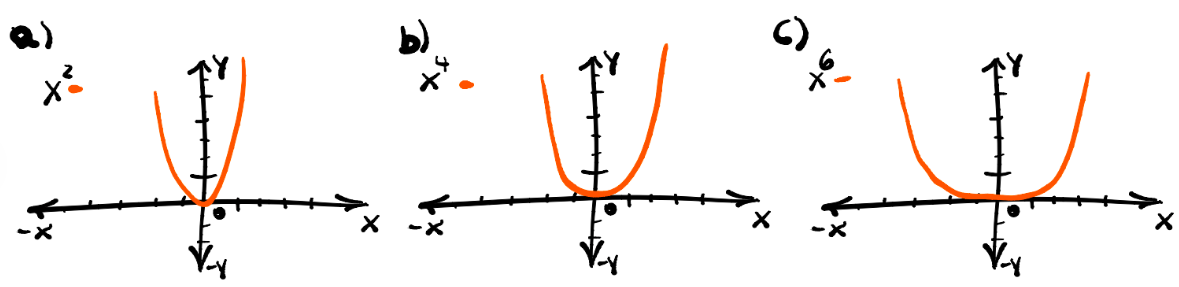
\includegraphics[scale=0.52]{fnpares.png}
\caption[Ejemplo funciones pares.]{Ejemplo funciones pares. a) Es la función cuadrática y en los casos b) y c) se ve como se va aplanando la región que pasa por el origen del plano, al igual que en el caso de los exponentes impares.} \label{fnpar}
\end{figure}
\end{center}

A estas funciones se debe sumar las variantes de las traslaciones, si se suma o resta una constante dentro o fuera del término principal, $x^{n}\pm c$ o $(x\pm c)^{n}+d$. \\
Por el momento, entraremos solo en el caso $x^{n}$ y debemos descifrar su comportamiento. En las figuras (\ref{fnimp}) y (\ref{fnpar}) se muestran todas las funciones cuando pasan por el origen, es decir, que los valores que toman los $x_{i}$ son muy bajos, pero ¿Qué ocurre cuando $x$ es muy grande? Lo que nos dirá esta respuesta es como se comporta la función muy lejos del origen.\\
El tomar valores altos del dominio de la función, es decir, que $x\longrightarrow +\infty$ o $x\longrightarrow -\infty$ hace ver como se comporta la función en \textbf{los extremos}.

\begin{mydef}
\label{extrefn0}
\textbf{Comportamiento de los extremos.} Cuando $x\longrightarrow\pm\infty$ la gráfica de una función polinomial\footnote{El símbolo $\rightarrow$ significa `tiende'. Es ponerse en caso en que la variable toma valores muy grandes.}
\begin{eqnarray*}
f(x)&=&a_{n}x^{n}+a_{n-1}x^{n-1}+a_{n-2}x^{n-2}+\cdots +a_{0} \\
\end{eqnarray*}
se asemeja a la gráfica $f(x)=a_{n}x^{n}$. Esto se debe a que los términos que le siguen aportan muy poco a la gráfica, en consecuencia la alteran muy poco.
\end{mydef}

\begin{myexample}
Sea $f(x)=7x^{3}+5x-20$, mostrar a que gráfica se asemeja esta función.
\begin{eqnarray*}
f(x)&=& 7x^{3}+5x-20 \\
f(x)&=& x^{3}\left(7+\dfrac{5x}{x^{3}}-\dfrac{20}{x^{3}} \right)\\
f(x)&=& x^{3}\left(7+\dfrac{5}{x^{2}} -\dfrac{20}{x^{3}}\right) \hspace{8px} x\longrightarrow \pm\infty\\
f(x)&=& 7x^{3}
\end{eqnarray*}
\end{myexample}
Visto el ejemplo anterior, se puede tener cuatro posibilidades en los extremos y dependen si el exponente es par o impar. Si consideramos el polinomio de la forma definida en (\ref{extrefn0}) y usando la aproximación del coeficiente principal obtenemos la siguiente información de la función polinomial.
\begin{table}[h!]
\begin{center}
		\begin{tabular}{|c|c|c|}
		\hline
		& $a_{n}<0$ & $a_{n}>0$ \\ 
		\hline
		Exponente par & $f(x<0)\longrightarrow -\infty$, $f(x>0)\longrightarrow -\infty$ &  $f(x<0)\longrightarrow \infty$, $f(x>0)\longrightarrow \infty$ \\
		\hline
		Exponente impar & $f(x<0)\longrightarrow \infty$, $f(x>0)\longrightarrow -\infty$ &  $f(x<0)\longrightarrow -\infty$, $f(x>0)\longrightarrow \infty$ \\
		\hline
		\end{tabular}
		\caption[Tabla de los extremos de una función polinomial.]{Tabla de los extremos de una función polinomial.}
\end{center}
\end{table}


\section{Funciones racionales}
\label{funrac0}
%300
Al igual que los números, los polinomios tienen sus operaciones y forman nuevas funciones, para el caso de la división son las funciones racionales. \\

\begin{mydef}
\textbf{Función racional. }Una función racional $y=f(x)$ es una función que tiene la forma:
\begin{eqnarray}
f(x)=\dfrac{P(x)}{Q(x)}
\end{eqnarray}
en donde $P(x)$ y $Q(x)$ son funciones polinomiales. Además, el denominador debe seer distinto de cero, $Q(x)\neq 0$.
\end{mydef}

Al momento de graficar las funciones racionales no es tan trivial, por lo que hay que sumar herramientas a las ya conocidas (Simetrías, intersecciones con los ejes, desplazamiento, etc.) para modelar las funciones, es por ellos que entraremos en detalle con las \textit{asíntotas}.\\

Una asíntota es una función lineal (una recta) que se aproxima de forma continua a la gráfica de una función $f(x)$, en otras palabras, la función $f(x)$ tiende al valor de la asíntota. La notación que introduciremos cuando $x$ se aproxima a un número $a$ o tiende a $\pm\infty$ es la siguiente:
\begin{itemize}
	\item $x\rightarrow a^{-}$, la variable $x$ tiende a $a$ desde la izquierda, es decir, a través de números más pequeños que $a$.\\
	\item $x\rightarrow a^{+}$, la variable $x$ tiende a $a$ desde la derecha, es decir, a través de números más grandes que $a$.\\
	\item $x\rightarrow a$, la variable $x$ tiende a $a$ desde la derecha y la izquierda.\\
	\item $x\rightarrow -\infty$, la variable $x$ tiende a $-\infty$, es decir, se vuelve no acotado en dirección negativa.\\
	\item $x\rightarrow \infty$, la variable $x$ tiende a $\infty$, es decir, se vuelve no acotado en dirección positiva.\\
\end{itemize}

\subsection{Asíntotas verticales}
Ocuparemos la notación introducida para definir los casos de asíntotas. Aquí veremos dos casos, horizontales y verticales. Como su nombre lo dice, las asíntotas verticales es una línea vertical que cruza por el eje $x$ y que nunca toca a la gráfica.

\begin{mydef}
\label{asintvert}
\textbf{Asíntotas verticales. } Se dice que una recta $x=a$ es una asíntota vertical de la gráfica de una función $f(x)$, si se cumple al menos una de estas seis condiciones:
\begin{itemize}
	\item $f(x)\rightarrow -\infty$ cuando $x\rightarrow a^{-}$ \\
	\item $f(x)\rightarrow -\infty$ cuando $x\rightarrow a^{+}$ \\
	\item $f(x)\rightarrow -\infty$ cuando $x\rightarrow a$ \\
	\item $f(x)\rightarrow +\infty$ cuando $x\rightarrow a^{-}$ \\
	\item $f(x)\rightarrow +\infty$ cuando $x\rightarrow a^{+}$ \\
	\item $f(x)\rightarrow +\infty$ cuando $x\rightarrow a$ \\
\end{itemize}
\end{mydef}

La definición (\ref{asintvert}) explica que cuando uno se acerca a las asíntotas, se puede hacer por la izquierda o por la derecha. Luego de acercarse por ambos lados puede darse el caso en que coincidan, entonces nace el concepto de una \textit{función continua} en el punto que uno se acerca. Si la función tiene una asíntota es una función discontinua, en palabras simples, es una función continua si puedo dibujar la gráfica sin levantar el lápiz.

 \begin{center}
\begin{figure}[h!]
\centering
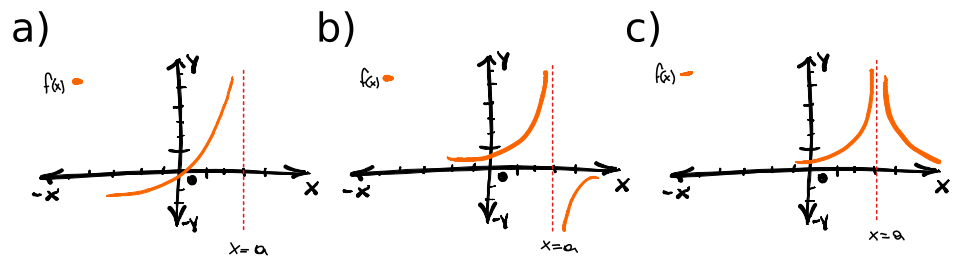
\includegraphics[scale=0.6]{asintvert.png}
\caption[Asíntotas verticales.]{Asíntotas verticales. a) Se ve en la gráfica que cuando me acerco por la izquierda la función tiende a $+\infty$, es decir, que $f(x)\rightarrow +\infty$ cuando $x\rightarrow a^{-}$.  b) $f(x)\rightarrow +\infty$ cuando $x\rightarrow a^{-}$ y $f(x)\rightarrow -\infty$ cuando $x\rightarrow a^{+}$. c) $f(x)\rightarrow \infty$ cuando $x\rightarrow a$. } \label{asintvert0}
\end{figure}
\end{center}

Ahora, ¿Las funciones de la figura (\ref{asintvert0}) son continuas?. La respuesta es si y no ¿Como?, si uno analiza la función completa claro que no es continua, porque tiene una asíntota de por medio, pero si uno toma un solo tramo (por ejemplo los casos b y c) de las funciones si lo son. Entonces la conclusión es que la función $f(x)$ es continua o discontinua según el tramo que se analice.

\subsubsection{Determinación de asíntotas verticales}

Para determinar las asíntotas se debe analizar la función racional de formar general
\begin{eqnarray}
\dfrac{P(x)}{Q(x)}=\dfrac{a_{n}x^{n}+a_{n-1}x^{x-1}+\cdots +a_{1}x+a_{0}}{b_{m}x^{m}+b_{m-1}x^{m-1}+\cdots + b_{1}x+b_{0}}
\label{fracpol}
\end{eqnarray}

Ahora supongamos que los polinomios $P(x)$ y $Q(x)$ de la ecuación (\ref{fracpol}) no tienen factores comunes (que no se pueden simplificar más). En este caso: \\

\textit{Si a es un número real tal que Q(a)=0, la recta x=a es una asíntota vertical de la gráfica de f(x).}\\

Entonces las soluciones de la ecuación del polinomio $Q(x)$ son las asíntotas verticales. Como el polinomio $Q(x)$ puede tener hasta $m$ raíces reales, entonces la gráfica puede tener hasta $m$ asíntotas verticales 
\begin{myexample}
Sea $f(x)$ una función definida en los números reales. Encontrar las asíntotas verticales de $f(x)$.
\begin{eqnarray*}
f(x)=\dfrac{P(x)}{Q(x)}&=&\dfrac{x^{2}+2}{x-2} \\
&=& x-2=0\\
x &=& 2
\end{eqnarray*}
$f(x)$ tiene una asíntota en $x=2$.

 \begin{center}
\begin{figure}[h!]
\centering
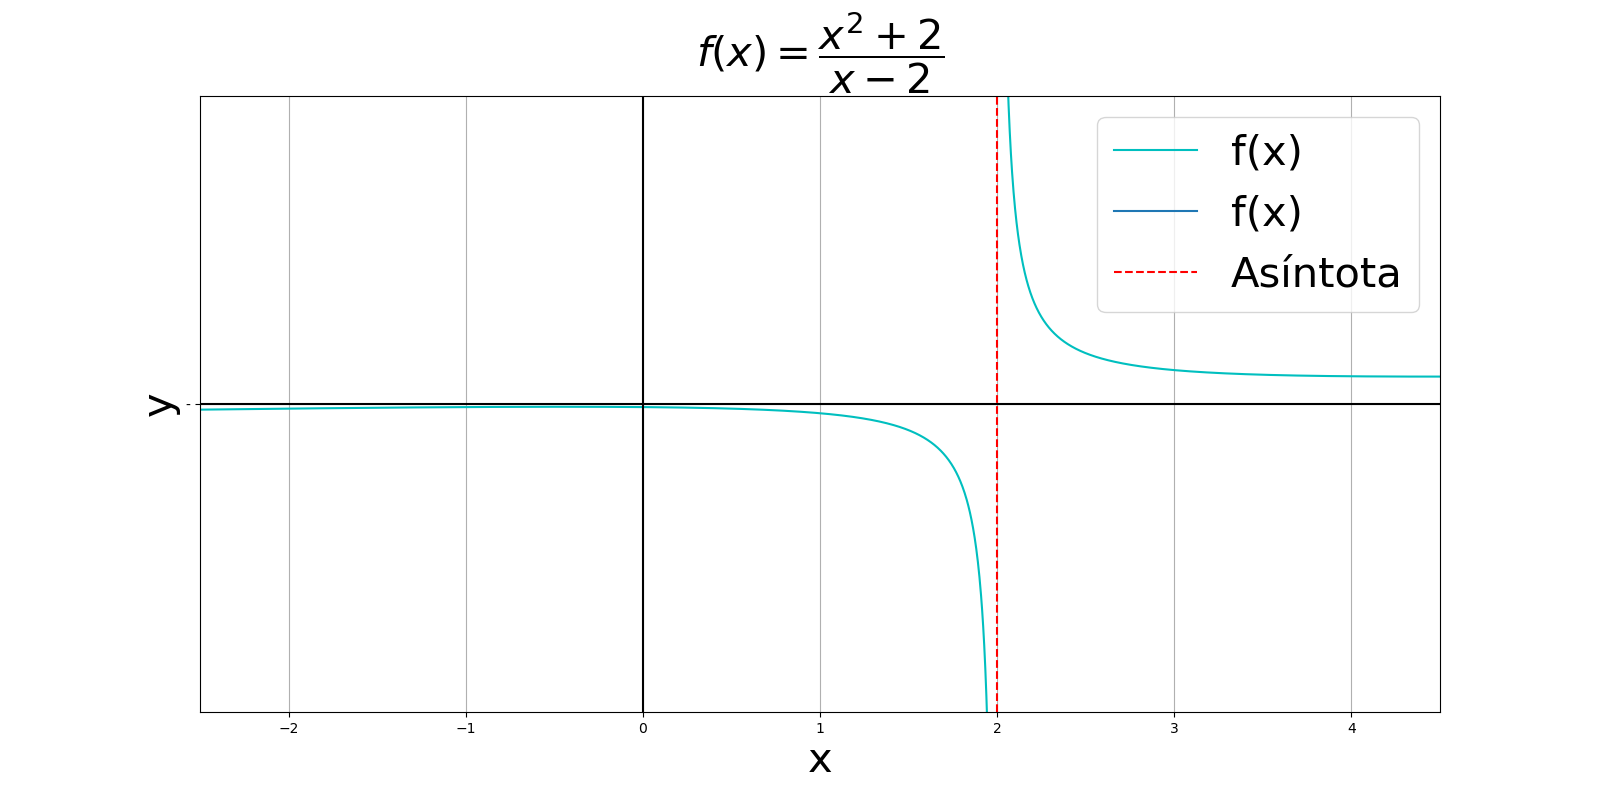
\includegraphics[scale=0.30]{asintver.png}
\caption{Gráfica de la función $f(x)$ con su asíntota en $x=2$.} \label{asintvert1}
\end{figure}
\end{center}
\end{myexample}

\subsection{Asíntotas horizontales}
Al igual que el caso vertical, existen asíntotas horizontales, pero ahora es una recta de valor constante. En este tipo de asíntotas muestran una diferencia con las verticales y es que se puede cruzar por la grafica.

\begin{mydef}
\textbf{Asíntotas horizontales. } Se dice que una recta $y=c$ es una asíntota horizontal de la gráfica de una función $f(x)$, si
\begin{itemize}
	\item $f(x)\rightarrow c$ cuando $x\rightarrow -\infty $ o si $f(x)\rightarrow c$ cuando $x\rightarrow +\infty $
\end{itemize}
\end{mydef}


\subsubsection{Determinación de asíntotas horizontales}
 Para el cálculo de las asíntotas horizontales se debe recurrir nuevamente al polinomio (\ref{fracpol}) con el detalle visto en la definición (\ref{extrefn0}). Recordando la definición, nos dice que a valores muy grandes de $x$ ($x\rightarrow \pm\infty$) la gráfica tiene la forma del término con el grado más alto del polinomio. Entonces, como los grados menores no aportan en los extremos, se reduce la expresión racional al primer termino del numerador y denominador. 

\begin{eqnarray}
f(x)&=&\dfrac{a_{n}x^{n}+a_{n-1}x^{x-1}+\cdots +a_{1}x+a_{0}}{b_{m}x^{m}+b_{m-1}x^{m-1}+\cdots + b_{1}x+b_{0}}\nonumber\\
&\approx &\dfrac{a_{n}x^{n}}{b_{m}x^{m}}\nonumber\\
&\approx & \dfrac{a_{n}}{b_{m}}x^{n-m}
\label{asinh0}
\end{eqnarray}

De la ecuación (\ref{asinh0}) se desprenden 3 casos:\\

\noindent a) Si $n=m$, $f(x)\approx \dfrac{a_{n}}{b_{m}}x^{n-m}\rightarrow \dfrac{a_{n}}{b_{m}}$ cuando $x\rightarrow \pm\infty$\\

\noindent b) Si $n<m$, $f(x)\approx \dfrac{a_{n}}{b_{m}}x^{n-m}= \dfrac{a_{n}}{b_{m}x^{n-m}}\rightarrow 0$ cuando $x\rightarrow \pm\infty$\\

\noindent c) Si $n>m$, $f(x)\approx \dfrac{a_{n}}{b_{m}}x^{n-m}= \dfrac{a_{n}x^{n-m}}{b_{m}}\rightarrow \infty$ cuando $x\rightarrow \pm\infty$\\

En resumen, el caso a) la asíntota es una recta horizontal donde $y= a_{n}/b_{m}$, el b) la asíntota es una recta $y=0$ y el caso c) no hay asíntota, pues diverge (se va a infinito) la función.
\begin{myexample}
Sea $f(x)$ una función definida en los números reales. Calcule la asíntota horizontal:
\begin{eqnarray*}
f(x)&=&\dfrac{8x}{x^{2}-2x+1}\\
&=&\dfrac{8x}{x^{2}\left(1-2\dfrac{1}{x}+\dfrac{1}{x^{2}}\right) }\\
&=&\dfrac{8x}{x^{2} }\\
&=&\dfrac{8}{x}, \hspace{10px} x\rightarrow \infty\\
y &=& 0 
\end{eqnarray*}

 \begin{center}
\begin{figure}[h!]
\centering
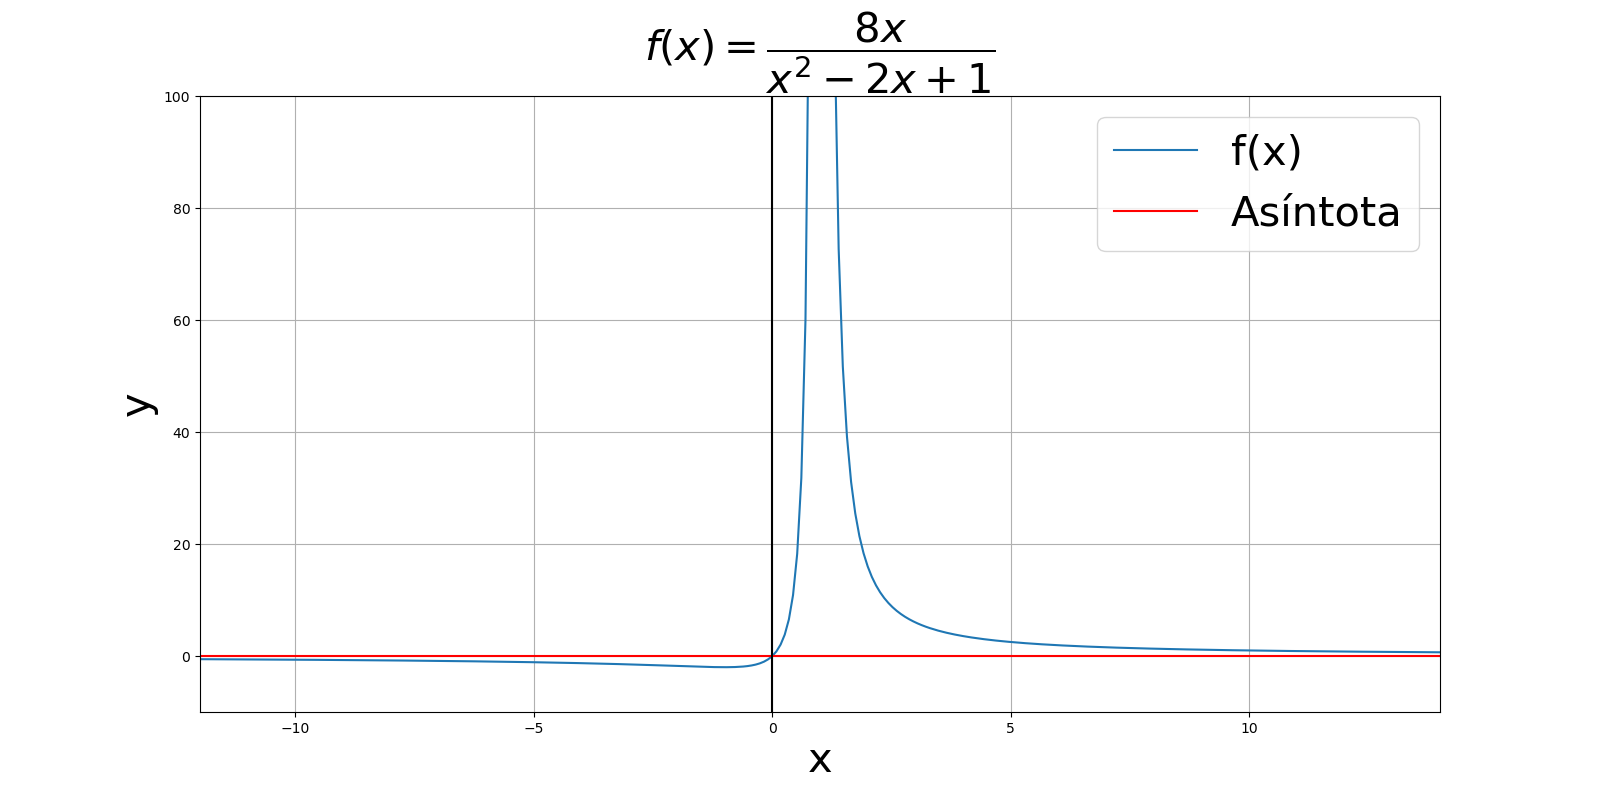
\includegraphics[scale=0.3]{asinth.png}
\caption[Gráfica de la función $f(x)$ con su asíntota horizontal en $y=0$.]{Gráfica de la función $f(x)$ con su asíntota horizontal en $y=0$. Notar que la función tiene una asíntota vertical, pero en este caso no es calculada.} \label{asintvert1}
\end{figure}
\end{center}
\end{myexample}
\newpage
\section{Funciones exponenciales}
En las secciones anteriores la variable es elevada a un número entero o decimal, para este caso veremos cuando un número es  elevado a la incógnita
\begin{mydef}
\textbf{Función exponencial.} Si $b>0$ y $b\neq 1$, una función exponencial $y=f(x)$ tiene la forma\\
\begin{eqnarray}
f(x)=b^{x}
\label{exp0}
\end{eqnarray}
El número b se llama base y x se llama exponente.
\end{mydef}
La condición en (\ref{exp0}) de que la base $b$ sea mayor que cero es para que $b^{x}$ sea un número real. Además, para el caso $x=0$ se tiene $f(0)=b^{0}=1$.\\

En la sección (\ref{exponentes}) se revisó las leyes de los exponentes enteros y decimales. Se puede mostrar que las leyes de los exponentes rigen a todos los exponentes reales. 
\begin{eqnarray}
x^{m}x^{n}&=&x^{m+n}\\
\left(\dfrac{x}{y}\right)^{n}&=&\dfrac{x^{n}}{y^{n}}\\
(x^{m})^{n}&=&x^{mn}\\
\dfrac{x^{m}}{x^{n}}&=&x^{m-n}\\
(xy)^{n}&=&x^{n}y^{n}
\end{eqnarray}
Reformularemos las ecuaciones ubicando la incógnita en el exponente. Notar que se necesita una base igual para poder realizar las operaciones entre exponentes. 

\begin{myexample}
Manipular la siguiente función
\begin{eqnarray}
f(x)=4^{-2x}=(4^{-2})^{x}=\left(\dfrac{1}{4^{2}} \right)^{x}=\left(\dfrac{1}{16} \right)^{x}
\end{eqnarray}
\end{myexample}

\subsection{Gráfica de una función exponencial}
Al momento de graficar las funciones exponenciales se desprenden dos casos. Esta división se hace dependiendo del valor de la base $b$. Un caso es para $b>1$ y el otro cuando $0<b<1$, se ve que para los números decimales $'0,...'$ elevado a $x$ tienen un comportamiento diferente a las expresiones con base más grande que uno. Además, se puede agregar que para ningún $x$ la expresión será cero, ya que el caso con menor exponente es $a^{0}=1$ (recordando que los exponentes negativos pasan a ser el parte del denominador), entonces las gráficas no intersectan el eje $x$.\\

En términos de las reflexiones, las funciones $b^{x}$ y $b^{-x}$ muestran ser opuestas en torno al eje $y$. Por otro lado, se menciona que las funciones exponenciales no traspasan el eje $x$ por lo que ese eje pasa a ser una asíntota horizontal para ambos casos ($y=0$). Utilizado la notación se expresa de la siguiente manera:
\begin{eqnarray}
b  > 1\nonumber\\
f(x)&=& b^{x}\rightarrow 0 \hspace{6px} cuando \hspace{6px} x\rightarrow -\infty\\
0< b  <1\nonumber\\
f(x)&=& b^{x}\rightarrow 0 \hspace{6px} cuando \hspace{6px} x\rightarrow \infty
\end{eqnarray}

 \begin{center}
\begin{figure}[h!]
\centering
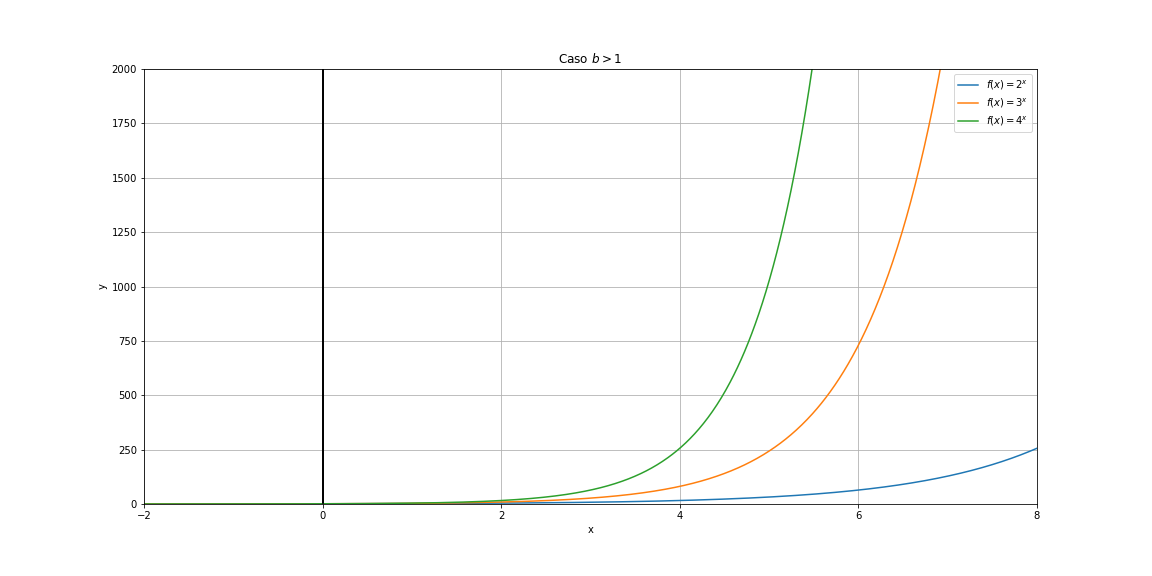
\includegraphics[scale=0.35]{expb0.png}
\caption[Gráfica de funciones exponenciales para el caso de la base $b>1$.]{Gráfica de funciones exponenciales para el caso de la base $b>1$. Se ve una función siempre creciente. El dominio son todos los reales y la imagen los reales positivos.} \label{expb0}
\end{figure}
\end{center}

 \begin{center}
\begin{figure}[h!]
\centering
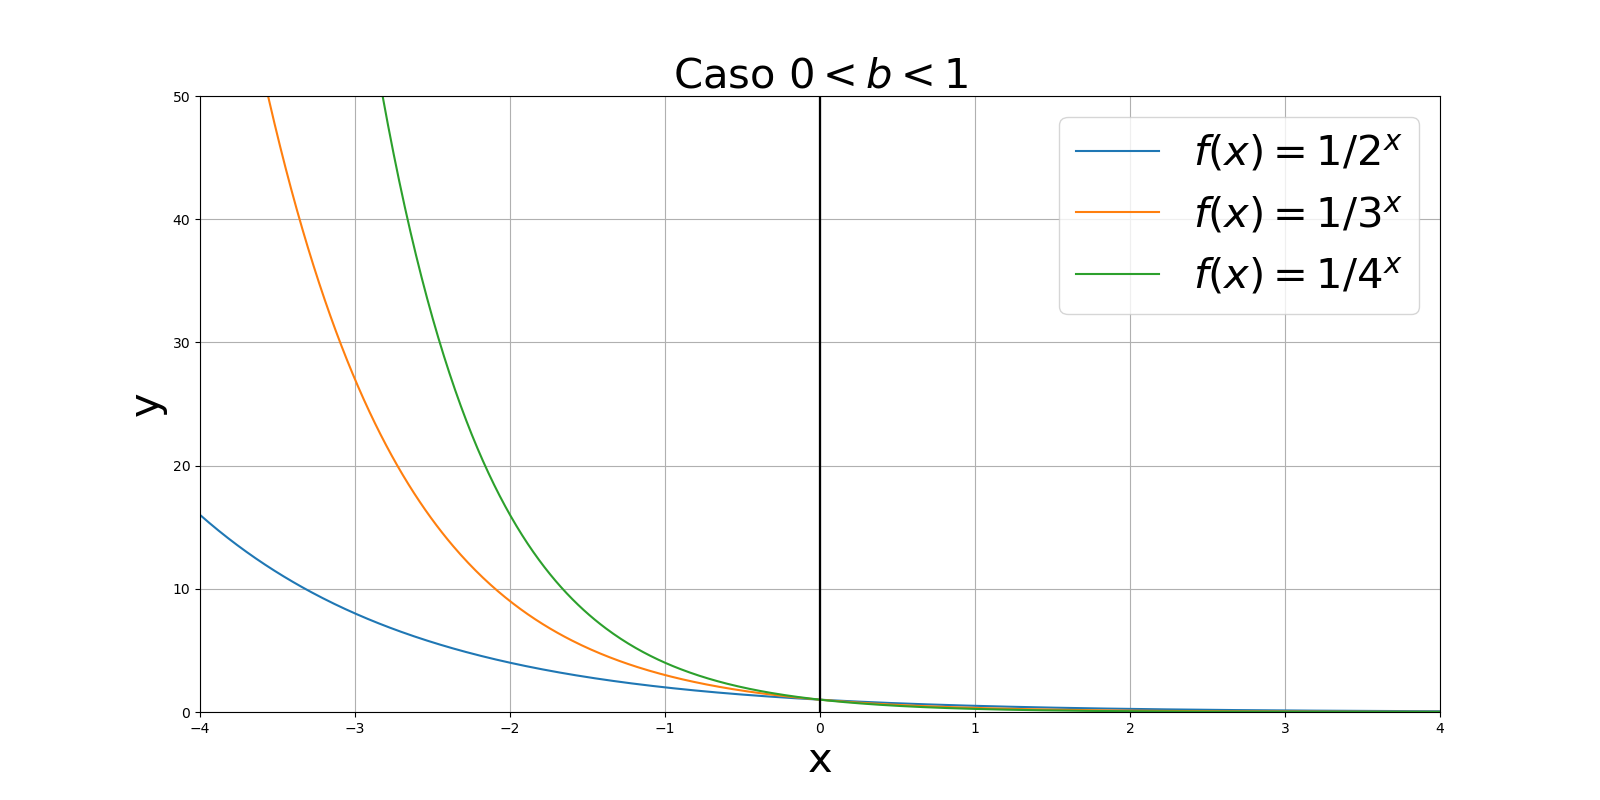
\includegraphics[scale=0.35]{expb1.png}
\caption[Gráfica de funciones exponenciales para el caso de la base $0<b<1$]{Gráfica de funciones exponenciales para el caso de la base $0<b<1$. Se ve una función siempre decreciente. El dominio son todos los reales y la imagen los reales positivos.} \label{expb1}
\end{figure}
\end{center}

De las figuras (\ref{expb0}) y (\ref{expb1}) se ve que las funciones exponenciales son uno a uno, continuas y que no cruzan el eje $x$. Adicionalmente, se puede dar el caso en que la función se desplaza, es decir, que al exponente se le suma un número, por ejemplo $4^{x+3}$ es una función desplazada de $4^{x}$. Dependiendo del caso, la función desplazada crece o decrece más rápido que la original.
\newpage
\subsection{Número e}

Un caso particular de base es el número $e$, que junto a $\pi$ son números particulares, ya que tienen decimales no repetitivos e infinitos. Una formar de representar estos números son series. Las series son sumas infinitas (se suman infinitos términos) de términos por medio de una expresión en común. 
\begin{eqnarray*}
e&=&1 + \dfrac{1}{1} + \dfrac{1}{1\cdot 2} + \dfrac{1}{1\cdot 2\cdot 3} + \dfrac{1}{1\cdot 2\cdot 3\cdot 4}+\cdots \\
&=&\dfrac{1}{0!} + \dfrac{1}{1!} + \dfrac{1}{ 2!} + \dfrac{1}{3!} + \dfrac{1}{4!}+\cdots \\
&=&\sum_{n=0}^{\infty}\dfrac{1}{n!}
\end{eqnarray*}
La notación $n!$ se le llama factorial y es la multiplicación de todos los números que hay desde $n$ hasta el $1$, el caso particular del del cero es $0!=1$. Para $n$ muy muy grandes ($n\rightarrow \infty$) el número $e$ tiende a la función
\begin{eqnarray*}
e&\rightarrow &\left(1+\dfrac{1}{x}\right)^{x} \\
e&=&2,7182818...
\end{eqnarray*} 
Por lo visto hay más de una forma para mostrar un simple número decimal (porque no deja de ser eso, un simple número decimal), pero muestra la importancia del número $e$ en la matemática.

\begin{mydef}
\textbf{Función exponencial natural. } Sea b la base de la función exponencial, entonces se elije $b=e$ y la función queda definida
\begin{eqnarray}
f(x)=e^{x}
\end{eqnarray}
\end{mydef}
Las gráficas de la función natural siguen la misma lógica de las figuras (\ref{expb0}) y (\ref{expb1}) cuando la base es $e$ y $1/e$ respectivamente. Puede ser desplazada verticalmente si se agrega una constante, por ejemplo $f(x)=c\pm e^{x}$.

Un caso en donde es muy usado el número $e$ es la en la función gaussiana, que en su forma más simple es $e^{-x^2}$. No cruza el eje $x$ y es simétrica  con respecto al eje $y$.
%Gráfica
\section{Funciones logarítmicas}

Las funciones exponenciales son uno a uno, por lo que debe existir una función vaya desde la imagen al dominio, es decir, una función inversa. Se introduce el concepto de logaritmo, por lo que la función logarítmica queda de la forma
\begin{mydef}
\textbf{Función logarítmica. } Con la base $b>0$, $b\neq 1$ se define por
\begin{eqnarray}
y=log_{b}(x), \hspace{10px} ssi \hspace{6px} x=b^{y}
\label{funlog0}
\end{eqnarray}
La abreviatura `ssi' es por la frase `si y solo si'. La función (\ref{funlog0})  se lee \textbf{y es el logaritmo de la base b que da como resultado x}.
\end{mydef}

En la función logarítmica $b>0$ no hay exponente $y$ que haga que la expresión $b^{y}$ sea menor que cero, en consecuencia, $x$ es mayor que cero. Entonces, el dominio de la función logarítmica son los números reales positivos.\\

Por el lado de las gráficas, ocurre igual que en las funciones exponenciales y se separan en dos casos según el valor de la base $b$. Se debe recordar que el dominio de las funciones exponenciales son todos los números reales y la imagen son los reales positivos. Entonces, como la función logarítmica es la inversa  de la función exponencial, los papeles se invierten.

 \begin{center}
\begin{figure}[h!]
\centering
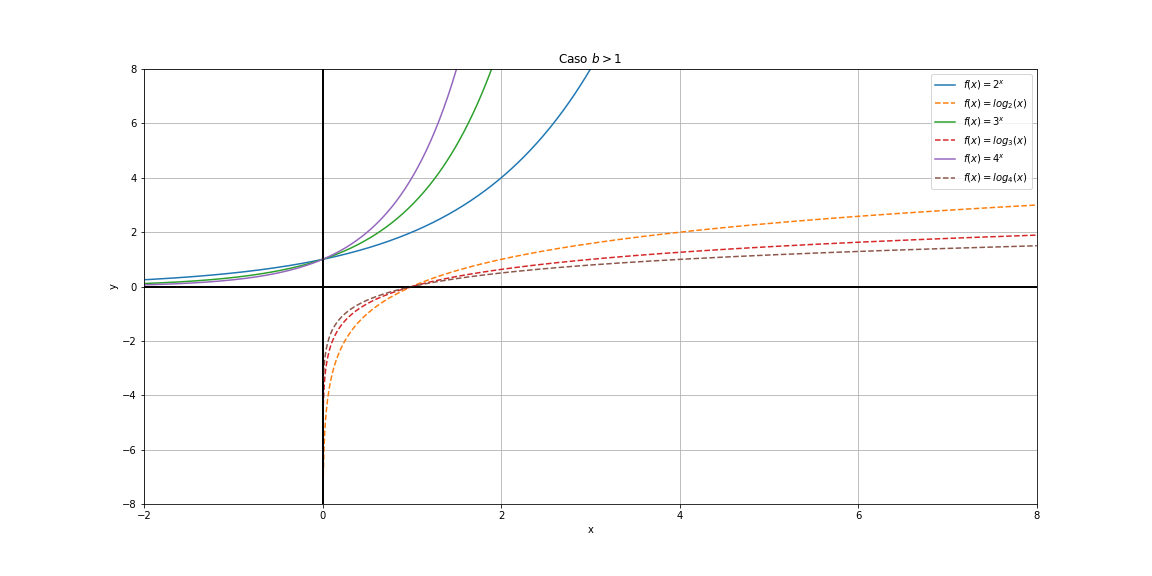
\includegraphics[scale=0.3]{logb0.png}
\caption[Gráfica de funciones logarítmicas para el caso de la base $b>1$]{Gráfica de funciones Logarítmicas para el caso de la base $b>1$. Notar que que se invierte el dominio con la imagen.} \label{logb0}
\end{figure}
\end{center}

 \begin{center}
\begin{figure}[h!]
\centering
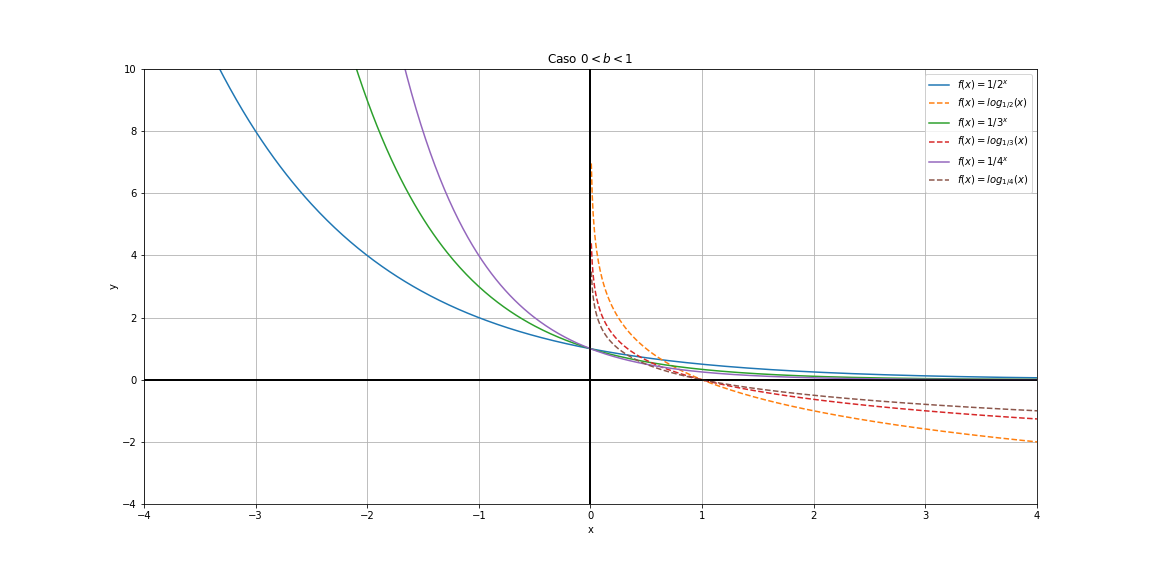
\includegraphics[scale=0.3]{logb1.png}
\caption[Gráfica de funciones logarítmicas para el caso de la base $0<b<1$]{Gráfica de funciones logarítmicas para el caso de la base $0<b<1$. Notar que se invierte el dominio con la imagen.} \label{logb1}
\end{figure}
\end{center}

Del las figuras (\ref{logb0}) y (\ref{logb1}) se ve que el eje $y$ es una asíntota vertical. Además, cuando el primer caso se va a $-\infty$ cuando se acerca el cero, mientras que para el segundo caso se va a $+\infty$. Entonces, algunas propiedades de la función logarítmica es que es uno a uno, es una función continua en el intervalo $]0,+\infty[$ y la intersección con el eje $x$ está en el punto $(1,0)$.\\

Hay un caso particular dentro del caso de la base $b>1$. Así como los logaritmos de base $10$ ($b=10$) se les llama comunes, a los logaritmos de base $e$ se les llama logaritmos naturales y su notación es $log_{e}(x)=ln(x)$. Entonces, ocurre que la expresión $ln(e)=1$ ya que $e^{1}=e$. Es una muestra más de que la función exponencial y la logarítmica son funciones inversas y las identidades quedan de la forma:
\begin{eqnarray}
x&=&e^{ln(x)}\\
y&=&ln(e^{y})
\end{eqnarray}
Lo que en palabras simples se traduce en que si tengo una función logarítmicas la puede eliminar con una función exponencial y viceversa. Para finalizar, mostraremos las leyes de los logaritmos
\newpage
\begin{mydef}
\textbf{Leyes de los logaritmos. } Para toda base $b>0$, $b\neq 1$, y para todos los números positivos $M$ y $N$.
\begin{itemize}
	\item $log_{b}(MN)=log_{b}(M)+log_{b}(N)$
	\item $log_{b}\left(\dfrac{M}{N}\right)=log_{b}(M)-log_{b}(N)$
	\item $log_{b}(M^{c})=c\cdot log_{b}(M)$, para cualquier número real c.\\
\end{itemize}
\end{mydef}

\begin{myexample}
Reducir el siguiente logaritmo:\\
\noindent\textit{i)}
\begin{eqnarray*}
ln(\sqrt{e})=ln(e^{1/2})=\dfrac{1}{2}ln(e)=\dfrac{1}{2}\cdot 1=\dfrac{1}{2}
\end{eqnarray*}
\noindent\textit{ii)}
\begin{eqnarray*}
log_{10}2\sqrt{2\sqrt{2\sqrt{2}}} &=&log_{10}2\left( 2\sqrt{2\sqrt{2}}\right)^{1/2}\\
 &=& log_{10}(2)+ log_{10}\left( 2\sqrt{2\sqrt{2}}\right)^{1/2}\\
 &=& log_{10}(2)+\dfrac{1}{2} log_{10}\left( 2\sqrt{2\sqrt{2}}\right)\\
  &=& log_{10}(2)+\dfrac{1}{2}\left[ log_{10}(2)+log_{10}\left( \sqrt{2\sqrt{2}}\right)\right]\\
    &=& log_{10}(2)+\dfrac{1}{2} log_{10}(2)+\dfrac{1}{2} log_{10}\left( \sqrt{2\sqrt{2}}\right)\\
    &=& log_{10}(2)+\dfrac{1}{2} log_{10}(2)+\dfrac{1}{2} log_{10}\left( 2\sqrt{2}\right)^{1/2}\\
     &=& \dfrac{3}{2} log_{10}(2)+\dfrac{1}{4} log_{10}\left( 2\sqrt{2}\right)\\
      &=& \dfrac{3}{2} log_{10}(2)+\dfrac{1}{4} log_{10}(2)+\dfrac{1}{4}log_{10}(2)^{1/2}\\
      &=& \dfrac{3}{2} log_{10}(2)+\dfrac{1}{4} log_{10}(2)+\dfrac{1}{8}log_{10}(2)\\
      &=& log_{10}(2)\left[\dfrac{3}{2}+\dfrac{1}{4}+\dfrac{1}{8} \right]\\
      &=& \dfrac{15}{8} log_{10}(2)\\
\end{eqnarray*}
\noindent\textit{iii)}
\begin{eqnarray*}
log_{10}\left(\dfrac{x^{4}y(w+z)}{wz} \right)&=& log_{10}\left(x^{4}y(w+z) \right)-log_{10}\left(wz \right)\\
&=& log_{10}(x^{4}y)+ log_{10}(w+z)-log_{10}\left(wz \right)\\
&=& log_{10}(x^{4})+log_{10}(y)+ log_{10}(w+z)-\left[ log_{10}(w)+log_{10}(z) \right]\\
&=& 4log_{10}(x)+log_{10}(y)+ log_{10}(w+z)-log_{10}(w)-log_{10}(z) \\
\end{eqnarray*}
\end{myexample}

\section{Ecuaciones exponenciales y logarítmicas}
Vistas las gráficas y propiedades de las funciones exponenciales y logarítmicas, ahora toca dar un paso adelante y es trabajar con las expresiones, pero agregando incógnitas. 

\begin{myexample}
Resolver la ecuación $e^{10x}=7$, encontrar el valor de x:\\

\noindent Sol: Primero, como la incógnita está en el exponente debemos encontrar una función que elimine la función exponencial, justamente es la logarítmica.
\begin{eqnarray*}
e^{10x}&=&7\\
10x&=&ln(7)\\
x&=&\dfrac{1}{10}ln(7)
\end{eqnarray*}
\end{myexample}

Una propiedad importante que viene de que las funciones logarítmicas y exponenciales son uno a uno es que $f(x_{1})=f(x_{2})$. Se puede utilizar esta herramienta para igualar términos y encontrar la incógnita.

\begin{mydef}
\textbf{Propiedades uno a uno de las funciones exponenciales y logarítmicas.} Sea $b$ la base de la función exponencial, con $b>0$, $b\neq 1$ y la función logarítmica $y=log_{b}(x)$. Se cumple que:
\begin{eqnarray}
Si\hspace{4px} b^{x_{1}} &=& b^{x_{2}},\hspace{4px} entonces\hspace{4px} x_{1}=x_{2}\\
Si\hspace{4px} log_{b}(x_{1})&=&log_{b}(x_{2}),\hspace{4px} entonces\hspace{4px} x_{1}=x_{2}
\end{eqnarray}
\end{mydef}

\begin{myexample}
Encontrar el valor de x de las siguientes ecuaciones:\\

\noindent\textit{i)}
\begin{eqnarray*}
7^{2(x+1)}&=&343\\
7^{2(x+1)}&=&7^{3}\\
2(x+1)&=&3\\
2x+2&=&3\\
2x&=&1\\
x&=&\dfrac{1}{2}
\end{eqnarray*}
\end{myexample}
\noindent\textit{ii)}
\begin{eqnarray*}
ln(2)+ln(4x-1)&=&ln(2x+5)\\
ln(2(4x-1))&=&ln(2x+5)\\
2(4x-1)&=&2x+5\\
8x-2&=&2x+5\\
6x&=&7\\
6x&=&7\\
x&=&\dfrac{7}{6}\\
\end{eqnarray*}

\section{Modelos matemáticos exponenciales y logarítmicos}

El paso que corona los conceptos vistos en las secciones anteriores, son los modelos matemáticos que se usan con estas funciones. Primero, para entender lo que es un modelo en palabras simples, es una expresión que \textit{intenta} describir matemáticamente un fenómeno. Este suceso no tiene por qué ser representando al $100\%$ por el modelo, porque puede estar echo para hacer cálculos futuros o tener una idea simple de lo que ocurre. Los modelos pueden ser tan simples o tan complejos como uno quiera y un factor que ayuda a los modelos son los \textit{parámetros}. Estas variables pueden ser constantes universalmente conocidas o números que cambian en el modelo según el caso que uno considere, dando un grado de realidad al modelo.

\subsection{Modelos matemáticos exponenciales}
Si hablamos de modelos exponenciales, es porque  la incógnita se encuentra en el exponente y un fenómeno descrito por estas funciones es el crecimiento de una población. Se debe agregar las constantes que condiciona la situación.
\begin{eqnarray}
P(t)=P_{0}e^{kt}, \hspace{6px} k>0 
\end{eqnarray} 
El término $P(t)$ nos dice que la incógnita es $t$, es decir, el tiempo. Por lo que el modelo nos dice cuanta población habrá en un tiempo determinado. La constante $P(0)$ se llama población inicial y se condiciona a la cantidad población que hay en el tiempo cero ($t=0$). Por último, la constante $k$ se llama tasa de crecimiento y nos dice que tan rápido crece, notar que si $k<0$ sería de decrecimiento. 
\newpage
\begin{myexample}
La bacteria Escherichia coli (E. coli) duplica su población en 20 minutos. Usar el modelo exponencial para calcular la población de bacterias después de 6 horas.\\

\noindent Sol: Lo primero en todo problema es asegurarse que todos los datos estén en la misma unidad de medida, entonces pasaremos los minutos a horas. Tiempo de duplicación de población $20min=1/3h$. Por otro lado, en este problema no se especifica nada sobre la población inicial, por lo que la dejaremos con el símbolo.\\

Notar que en $t=1/3$ la bacteria duplica su población, es decir, $P(1/3)=2P_{0}$ y reemplazando $t$ en el modelo queda:
\begin{eqnarray*}
P(1/3)&=&  2P_{0}\\
P_{0}e^{k/3}&=&2P_{0}\\
e^{k/3}&=&2\\
\dfrac{k}{3}&=&ln(2)\\
k&=&3\cdot ln(2)\\
\end{eqnarray*}
Ahora ya tenemos el valor de la constante $k$, entonces lo reemplazamos en el modelo
\begin{eqnarray*}
P(t)&=&P_{0}e^{3\cdot ln(2)\cdot t}\\
P(t=6)&=&P_{0}e^{3\cdot ln(2)\cdot 6}\\
P(t=6)&=&P_{0}e^{18\cdot ln(2) }\\
P(t=6)&=&P_{0}\cdot 262144
\end{eqnarray*}
Ahora uno puede poner casos particulares de la población inicial ($P_{0}$) y multiplicarlo por $262144$, que es la población de la bacteria luego de $6$ $horas$.
\end{myexample}

\begin{myexample}
Se necesita estudiar el crecimiento de dos tipos de bacterias, $P_{1}$ y $P_{2}$. La primera alcanza la población de $10.000$ en $4$ horas y la segunda comienza con el doble de la población respecto a la primera, además la segunda alcanza la población de $10.000$ en $3$ horas. Con el modelo exponencial encuentre la población inicial ($P_{0}$) de cada bacteria. Se asume el parámetro de crecimiento $k$ es el mismo para ambas bacterias
\end{myexample}
Expresiones para ambas bacterias:
\begin{eqnarray}
P_{1}(t)= P_{0}e^{kt} &y& P_{2}=2P_{0}e^{kt}
\label{bac}
\end{eqnarray}
Expresiones en que la población de ambas bacterias es de $10.000$:
\begin{eqnarray*}
P_{1}(t=4)=10000 &y& P_{2}(t=3)=10000 \\
P_{0}e^{4k}&=&2P_{0}e^{3k}=10000\\
e^{4k}&=&2e^{3k}\hspace*{90px} / \cdot e^{-3k}\\
e^{k}&=&2\hspace*{105px} / ln()\\
ln(e^{k})&=&ln(2)\\
k&=& ln(2)
\end{eqnarray*}
Encontrado el parámetro k (que es el mismo para ambas bacterias), se reemplaza en (\ref{bac}) y se obtiene:
\begin{eqnarray*}
P_{1}(t)= P_{0}e^{ln(2)t} &y& P_{2}=2P_{0}e^{ln(2)t}
\end{eqnarray*}
y las expresiones cuando alcanzar las $10000$ bacterias son:
\begin{eqnarray*}
10000= P_{0}e^{4\cdot ln(2)} &y& 10000=2P_{0}e^{3\cdot ln(2)}\\
10000= P_{0}e^{4\cdot ln(2)} &y& 5000=P_{0}e^{3\cdot ln(2)}\\
10000= P_{0}e^{ ln(16)} &y& 5000=P_{0}e^{ln(8)}\\
P_{0}=\dfrac{10000}{e^{ln(16)}} &y& P_{0}=\dfrac{5000}{e^{ln(8)}}\\
P_{0}&=&625
\end{eqnarray*}
Como la población inicial es $P_{0}=625$ unidades. Entonces la bacteria uno, $P_{1}$, comenzó con $625$ de población inicial y la bacteria dos, $P_{2}$, con $1250$ unidades.
\subsection{Modelos matemáticos logarítmicos}

Una aplicación muy interesante donde aplicar los logaritmos, en base 10 en este caso, es en la escala de Ricther. Esta escala compara las energías de distintos sismos. 
\begin{eqnarray}
M=log_{10}\left(\dfrac{A}{A_{0}}\right)
\end{eqnarray}
M es la magnitud del sismo y $A_{0}$ es una amplitud de referencia que corresponde a la magnitud $M=0$

\begin{mydef}
En el año 1960 en la ciudad de Valdivia en Chile, ocurrió un terremoto de grado $9,6$ en la escala de Richter. En el año 2010 en Concepción en Chile, hubo un terremoto de grado $8,8$. Entonces ¿Cuántas veces más intenso fue el terremoto del año 1960 con respecto al del 2010?\\

\noindent Sol: Primero definimos las expresiones que le corresponde a cada terremoto
\begin{eqnarray*}
9,6=log_{10}\left(\dfrac{A}{A_{0}}\right)_{1960} \hspace{5px} y \hspace{5px}8,8=log_{10}\left(\dfrac{A}{A_{0}}\right)_{2010}
\end{eqnarray*}
Si se aplica la función logarítmica los términos queda de la forma
\begin{eqnarray*}
\left(\dfrac{A}{A_{0}}\right)_{1960}&=&10^{9,6} \hspace{5px} y \hspace{5px} \left(\dfrac{A}{A_{0}}\right)_{2010} = 10^{8,8}\\
\left(\dfrac{A}{A_{0}}\right)_{1960}&=&10^{9,6}=10^{8,8}\cdot 10^{0,8}\\
\left(\dfrac{A}{A_{0}}\right)_{1960}&=&10^{0,8}\left(\dfrac{A}{A_{0}}\right)_{2010}\\
\left(\dfrac{A}{A_{0}}\right)_{1960}&\approx & 6,3\left(\dfrac{A}{A_{0}}\right)_{2010}
\end{eqnarray*}
Entonces, el terremoto del año $1960$ en Valdivia fue más de $6$ veces más fuerte que el terremoto del año $2010$ en Concepción.
\end{mydef}

\subsection{Escalas logarítmicas y lineales}
Al ver las funciones logarítmicas y exponenciales se puede notar que no siempre es lo más optimo ocupar la \textit{escala usual}.  Comúnmente se una la escala lineal en los gráficos, que tiene la misma distancia entre los puntos que delimitan el gráfico (la distancia que hay entre en 1 y el 2, es la misma que hay entre el 2 y el 3 y así sucesivamente). Hay otras escalas que representan mejor algunas funciones, como por ejemplo las logarítmicas. Esta escala tiene como etiquetas los números $10^{n}$, siendo $n$ un número entero positivo o negativo, por lo que la etiqueta es siempre positiva.\\
Como resumen de estas escalas, es que son importante o son útiles usarlas cuando el rango de los datos es muy amplia.\\

A continuación mostramos algunos ejemplos de diferentes funciones graficadas en cuatros escalas distintas. De izquierda a derecha y de arriba a abajo es: Escala lineal, escala logarítmica en $x$ o semilog en $x$ (esto quiere decir que se utiliza escala logarítmica solo en el eje $x$), escala logarítmica en $y$ o semilog $y$ y escala logarítmica (escala logarítmica tanto en $x$ como en $y$).\\



 \begin{center}
\begin{figure}[h!]
\centering
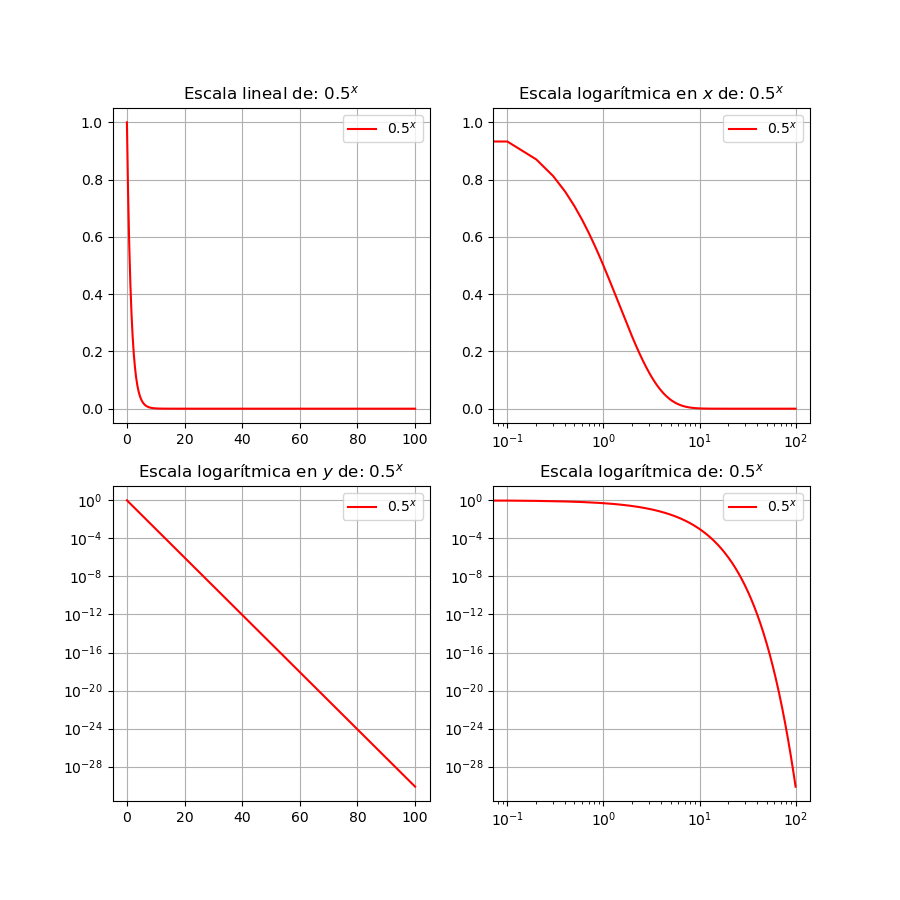
\includegraphics[scale=0.4]{Func0.png}
\caption[Cuatro escalas de la función $0.5^{x}$]{Cuatro escalas de la función $0.5^{x}$.} \label{func00}
\end{figure}
\end{center}

 \begin{center}
\begin{figure}[h!]
\centering
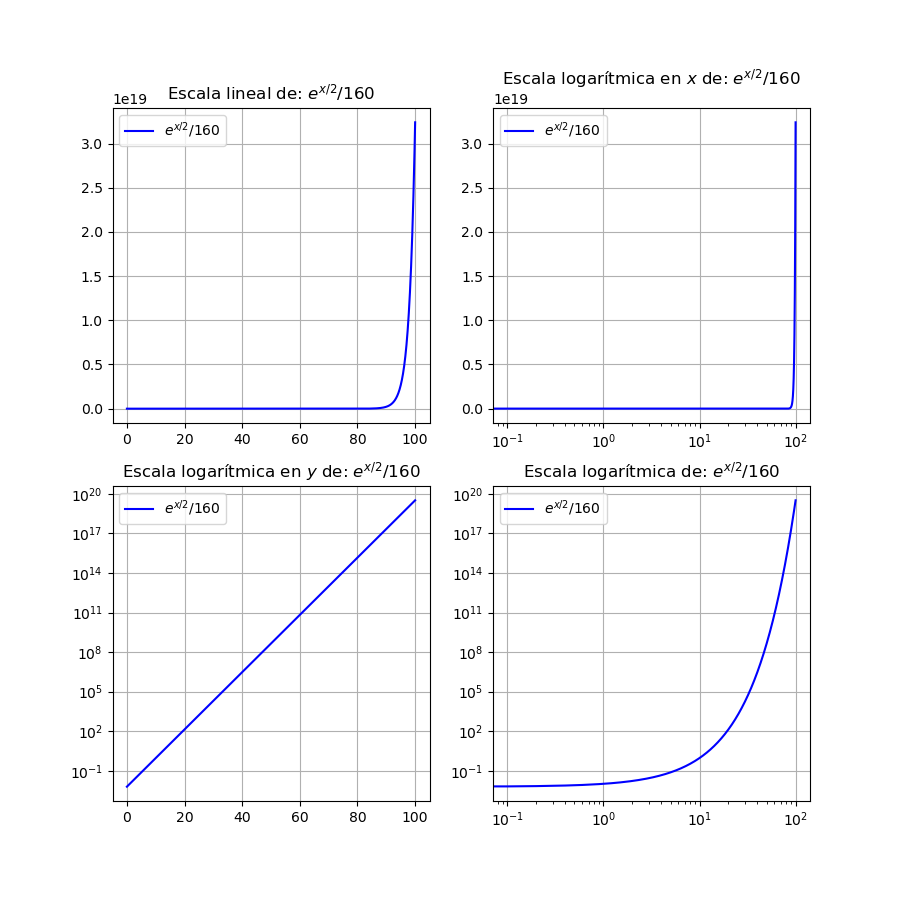
\includegraphics[scale=0.4]{Func1.png}
\caption[Cuatro escalas de la función $e^{x/2}/160$]{Cuatro escalas de la función $e^{x/2}/160$.} \label{func01}
\end{figure}
\end{center}

 \begin{center}
\begin{figure}[h!]
\centering
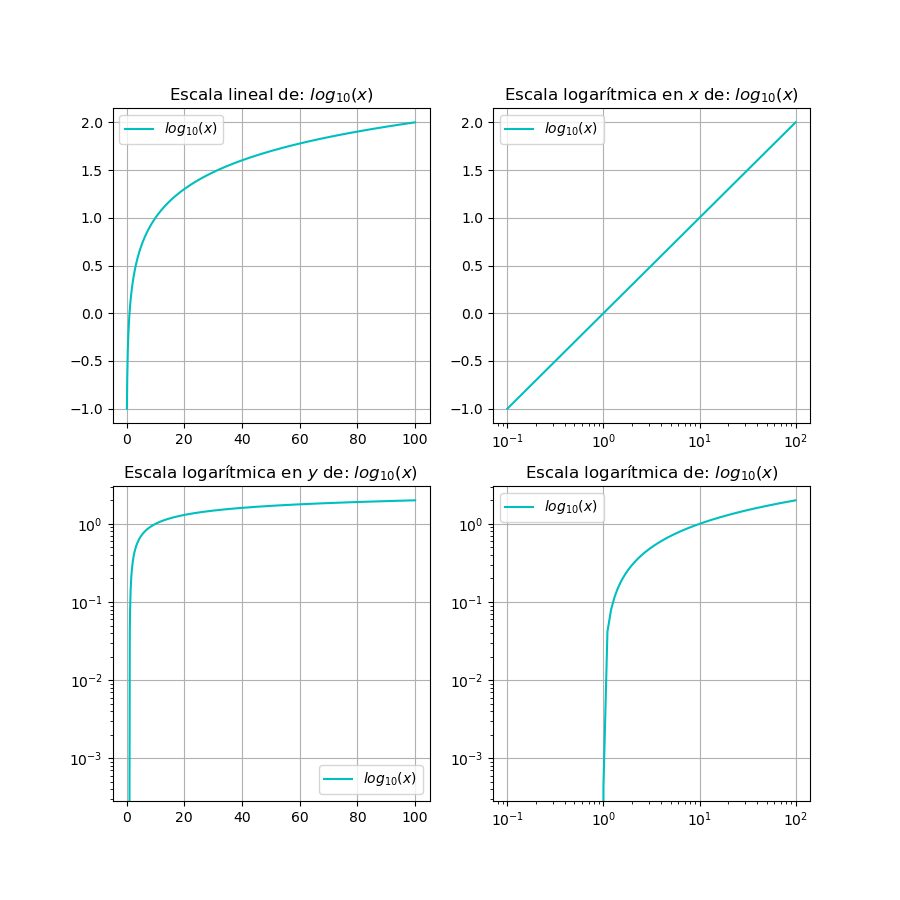
\includegraphics[scale=0.4]{Func2.png}
\caption[Cuatro escalas de la función $log_{10}(x)$]{Cuatro escalas de la función $log_{10}(x)$.} \label{func02}
\end{figure}
\end{center}

% \begin{center}
%\begin{figure}[h!]
%\centering
%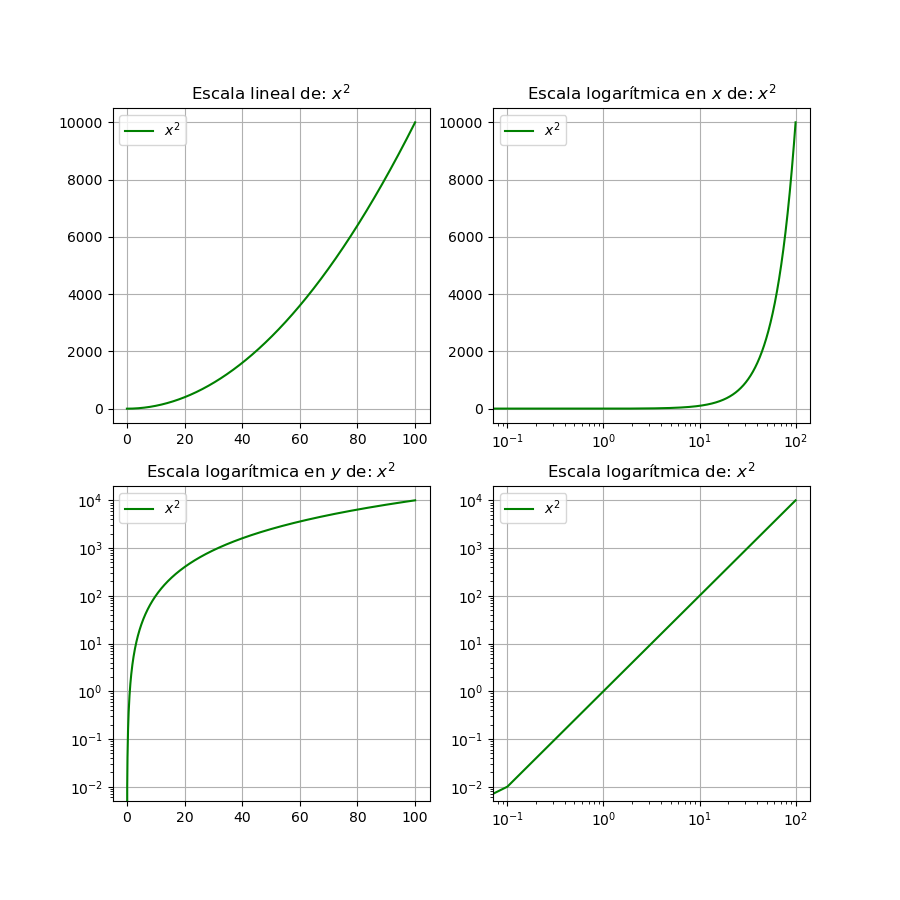
\includegraphics[scale=0.45]{Func3.png}
%\caption[Cuatro escalas de la función $x^{2}$]{Cuatro escalas de la función $x^{2}$.} \label{func03}
%\end{figure}
%\end{center}